\documentclass[12pt,a4paper]{report}
% Preamble packages
\usepackage[utf8]{inputenc}
\usepackage{acronym}
\usepackage{amssymb}
\usepackage{wrapfig}
\usepackage{amsmath}
\usepackage{graphicx}
\usepackage{epstopdf}
\usepackage{booktabs}
\usepackage{hyperref}
\hypersetup{
	colorlinks=true,
	linkcolor=blue,
	filecolor=magenta,     
	citecolor=blue, 
	urlcolor=blue,
}
\usepackage{float}
\usepackage{cleveref}
\usepackage[left=3.5cm,right=2.5cm,top=2.5cm,bottom=2.5cm]{geometry}
\usepackage{lineno}
\usepackage{comment}
\usepackage{natbib}
\usepackage{multicol}
\usepackage{xcolor}
\usepackage{amsfonts}
\usepackage{rotating}
\usepackage{multirow}
\usepackage{bm}
\usepackage[toc,page]{appendix}
\usepackage{ragged2e}
\usepackage{anyfontsize}
\usepackage{caption}
\usepackage{longtable}
%-----------------------------------------------------------------------



%---------------------------------------------------------------------
% Custom commands
\newcommand{\dedicationNamea}{My Mother}
\newcommand{\dedicationNameb}{My Father}

% Global definitions
\def\mytitle{Engunity X : AI-Powered SaaS Platform for Research, Code Generation and Data Analysis}

% Student names — approved 4-column table
\def\myname{
    \begin{table}[h]
        \centering
        \begin{tabular}{|c|l|l|l|}
            \hline
            Sr. No. & Name              & Roll No.          & Email ID                       \\ \hline
            1       & Shubh Shah       & 22UF17191AI053    & shubh.17191@sakec.ac.in       \\ \hline
            2       & Anurag Kumar     & 22UF17647AI027    & anurag.kumar17647@sakec.ac.in \\ \hline
            3       & Shreyash Mokani  & 22UF17269AI032    & shreyash.17269@sakec.ac.in    \\ \hline
            4       & Nigranth Shah    & 22UF17430AI051    & nigranth.17430@sakec.ac.in    \\ \hline
        \end{tabular}
        \label{tab:students}
    \end{table}
}

\def\mydegree{BACHELOR OF TECHNOLOGY}
\def\branch{ARTIFICIAL INTELLIGENCE AND DATA SCIENCE}
\def\mysupervisor{Dr. Rahul Pachade}
\def\myrollno{   }
\def\mydep{Department of Artificial Intelligence And Data Science}
\def\mydegreedate{MAY 2026}
\def\mycollege{Shah and Anchor Kutchhi Engineering College, Mumbai}

\setlength{\parskip}{0.5em} % Adjust the value as needed its the spacing between paragraphs

\begin{document}

\baselineskip=18pt plus1pt
\setcounter{secnumdepth}{3}
\setcounter{tocdepth}{3}
\pagenumbering{roman}

% Temporarily disable parskip for front matter
\newlength{\savedparskip}
\setlength{\savedparskip}{\parskip}
\setlength{\parskip}{0pt}

% Front matter
\thispagestyle{empty}
\begin{center}
    { \large {\bfseries {\ Engunity X : AI-Powered SaaS Platform for Research, Code Generation and Data Analysis}} \par}
\vspace{1\baselineskip}
    {\large \textbf{A} \par}
\vspace{0.5\baselineskip}
    {\large \textbf{DISSERTATION/REPORT} \par}
\vspace{0.5\baselineskip}
    {\textit{Submitted for fulfillment of the Requirement}\\
    \textit{For the award of the degree of}}\par
\vspace{\baselineskip}
    {\large \bf \mydegree \par}
\vspace{0.5\baselineskip}
{\large \textbf{In} \par}
\vspace{0.5\baselineskip}
    {\large \bf \branch \par}
\vspace{0.5\baselineskip}
    {\textit{Submitted by} \par}
\vspace{\baselineskip}
    \begin{table}[htbp]
\centering
\begin{tabular}{|c|l|l|l|}
\hline
\textbf{Sr. No.} & \textbf{Name} & \textbf{Roll No.} & \textbf{Email ID} \\ \hline
1 & Shubh Shah& 22UF17191AI053& shubh.17191@sakec.ac.in\\ \hline
2 & Anurag Kumar& 22UF17647AI027& anurag.kumar17647@sakec.ac.in\\ \hline
3 & Shreyash Mokani& 22UF17269AI032& shreyash.17269@sakec.ac.in\\ \hline
4 & Nigranth Shah& 22UF17430AI051& nigranth.17430@sakec.ac.in\\ \hline
\end{tabular}
\end{table}

    {Under the guidance of \par}
\vspace{\baselineskip}
    {{\large \bf Dr. Rahul Pachade} \par}
\vspace{0.5\baselineskip}
    {Associate Professor \par}
\vspace{\baselineskip}
    {\begin{figure}[!h]
	\centering
	
\includegraphics[width=35mm]{images/SAKEC_logo.png}
     \end{figure}
    }
    {\bf \MakeUppercase{\mydep} \par}
\vspace*{1ex}
   { \bf \uppercase{SHAH \& ANCHOR KUTCHHI ENGINEERING COLLEGE } }\\
   \vspace{-0.2 \baselineskip}
    {(An Autonomous Institute Affiliated to University of Mumbai) \par}
   
 {\bf \uppercase { MUMBAI - 400 088, MAHARASHTRA (India)  \par  \mydegreedate}}
 \end{center}
\addcontentsline{toc}{section}{Certificate} %CERTIFICATE
\thispagestyle{plain}

\begin{minipage}[c]{1mm}
            
\includegraphics[width=23mm]{images/SAKEC_logo.png}
        \end{minipage}
        \hfill
        \begin{minipage}[c]{126mm}
            \centering
            { \bf \large {Shah \& Anchor Kutchhi Engineering College  } }\\
   \vspace{-0.01 \baselineskip}
    {(An Autonomous Institute Affiliated to University of Mumbai) }
    { \bf \small {Mumbai-400 088, MAHARASHTRA (India)   } }\\
                
            
        \end{minipage}

\vspace{0.2\baselineskip}

\begin{center}
{\Large {\bf \uppercase{Certificate}}}
\end{center}
\vspace{\baselineskip}
\hrule
\vspace{2\baselineskip}

{It is my pleasure to certify that the following students worked under my supervision for the
B. Tech. 
    \begin{table}[htbp]
\centering
\begin{tabular}{|c|l|l|l|}
\hline
\textbf{Sr. No.} & \textbf{Name} & \textbf{Roll No.} & \textbf{Email ID} \\ \hline
1 & Shubh Shah& 22UF17191AI053& shubh.17191@sakec.ac.in\\ \hline
2 & Anurag Kumar& 22UF17647AI027& anurag.kumar17647@sakec.ac.in\\ \hline
3 & Shreyash Mokani& 22UF17269AI032& shreyash.17269@sakec.ac.in\\ \hline
4 & Nigranth Shah& 22UF17430AI051& nigranth.17430@sakec.ac.in\\ \hline
\end{tabular}
\end{table}
dissertation/Project Report entitled {\mytitle}{\textbf{\ }}and their work is of the level of requirement set up for the dissertation/Project Report in {\branch}  by Shah \& Anchor Kutchhi Engineering College, Mumbai.}


\bigskip

\begin{tabular}{p{0.5\textwidth}p{0.5\textwidth}}
Date:\ 07/05/2026 \\
\end{tabular}

\textsc{}{This is to certify that the above statement made by the candidates is correct to the best of my knowledge.}\par
\vspace{0.5\baselineskip}
{\mysupervisor} \par
{Associate Professor \par \mydep \par Shah \& Anchor Kutchhi Engineering College \par Mumbai -- 400 088, India}


\vspace{0.5\baselineskip}

{The viva-voice/Oral and Practical examination of B. Tech. in \branch,
has been held on \ May 2026}

\vspace{2\baselineskip}

\begin{tabular}{p{0.35\textwidth}p{0.35\textwidth}p{0.35\textwidth}}
\textbf{External Examiner} & \textbf{Internal Examiner} & \textbf{Guide Name}\\
\textit{} & \textit{} & \textit{(Dr. Rahul Pachade)}
\end{tabular}

\vspace{2\baselineskip}

\begin{tabular}{p{0.35\textwidth} p{0.35\textwidth} p{0.35\textwidth}}
    \textbf{I/C Head of Department} & \textbf{  Principal} & \textbf{College Seal} \\
    \textit{(Dr. Pravin Shinde)} & \textit{(Dr. Bhavesh Patel)} & \textit{}
\end{tabular}



\bigskip
\addcontentsline{toc}{section}{Candidate's Declaration}%CANDIDATE'S DECLARATION
\thispagestyle{empty}

\begin{center}
{\Large {\bf \uppercase{Candidate's Declaration}}}
\end{center}

\vspace{\baselineskip}
\hrule
\vspace{2\baselineskip}

We hereby declare that the work presented in the dissertation/Project Report entitled {{\mytitle}} for fulfillment of the requirement for the degree of B. Tech.\ in \branch and submitted to the \mydep~ at Shah \& Anchor Kutchhi Engineering College, Mumbai, is an authentic record of our own work carried out during the period from June 2025 to May 2026 under the supervision of {\mysupervisor} \par
\vspace{2\baselineskip}
The matter presented in this dissertation/Project Report has not been submitted elsewhere in part or fully to any other University or Institute for the award of any other degree.


\bigskip


\bigskip


\bigskip

{\textbf{Signature of the students \ \ \ \ \ \ }}

  \begin{table}[htbp]
\centering
\begin{tabular}{|c|l|l|l|l|}
\hline
\textbf{Sr. No.} & \textbf{Name} & \textbf{Roll No.} & \textbf{Email ID}  & Signature\\ \hline
1 & Shubh Shah& 22UF17191AI053& shubh.17191@sakec.ac.in&\\ \hline
2 & Anurag Kumar& 22UF17647AI027& anurag.kumar17647@sakec.ac.in&\\ \hline
3 & Shreyash Mokani& 22UF17269AI032& shreyash.17269@sakec.ac.in&\\ \hline
4 & Nigranth Shah& 22UF17430AI051& nigranth.17430@sakec.ac.in&\\ \hline
\end{tabular}
\end{table}
\addcontentsline{toc}{section}{Certificate of Plagiarism Check}
\thispagestyle{plain}

\begin{minipage}[c]{1mm}
            
\includegraphics[width=23mm]{images/SAKEC_logo.png}
        \end{minipage}
        \hfill
        \begin{minipage}[c]{126mm}
            \centering
            { \bf \large \mydep }\\
   \vspace{-0.01 \baselineskip}
    {(An Autonomous Institute Affiliated to University of Mumbai) }
        \end{minipage}

\vspace{0.2\baselineskip}

\begin{center}
{\Large {\bf \uppercase{CERTIFICATE OF PLAGIARISM CHECK}}}
\end{center}
\vspace{\baselineskip}
\hrule
\vspace{0.1\baselineskip}

\begin{center}
\begin{longtable} { |p{6cm}|p{8cm}|  }
\hline
\multicolumn{2}{|c|}{\textbf{CERTIFICATE OF PLAGIARISM CHECK}} \\
\hline
Title of the Dissertation/Report & \mytitle \\ 
\hline
Name of the Supervisor/Guide & \mysupervisor \\ 
\hline
Name of the Department & \mydep \\ 
\hline

Similar content (\%) identified &  9  \% \\ 
\hline
Acceptable Maximum Limit & 10  \% \\
\hline
Name of the Similarity tool used for Plagiarism Report &   Turnitin \\
\hline

Date of Verification &  16/05/2026 \\ 
\hline 

Name \& Sign of the DAIP Member & \\ \hline
Name \& Sign of Students & Shubh Shah, Anurag Kumar, Shreyash Mokani, Nigranth Shah \\ \hline
Name \& Sign of the Guide & \mysupervisor \\ \hline
\end{longtable}
\end{center}

\noindent
Shah \& Anchor Kutchhi Engineering College, Chembur \\
Date: \ 16/05/2026

\bigskip
\addcontentsline{toc}{section}{Dedication} % DEDICATION
\include{./front_matter/dedication}
\addcontentsline{toc}{section}{Acknowledgements} %ACKNOWLEDGEMENTS
\thispagestyle{empty}

\begin{center}
{\Large {\bf \uppercase{Acknowledgements}}}
\end{center}

\vspace{\baselineskip}
\hrule
\vspace{2\baselineskip}
We would like to express our heartfelt gratitude to all those who supported
and guided us throughout this project. We sincerely thank our project guide, Dr.\ Rahul Pachade, Associate Professor, Department of Artificial Intelligence and Data Science, for their valuable insights, constant encouragement, and for suggesting early in the project that we decouple the execution sandbox before any of the other services were built---a decision that saved significant refactoring time later.

We are grateful to the faculty of the Department of Artificial Intelligence and Data Science at Shah \& Anchor Kutchhi Engineering College for providing us with the necessary resources and knowledge. Special thanks to our peers for their support and collaboration, and to our families for their unwavering encouragement throughout this journey.

We also acknowledge the open-source communities behind FastAPI, Next.js, FAISS, sentence-transformers, FlashRank, EasyOCR, Ultralytics YOLOv8, Monaco Editor, XTerm.js, and GitPython, whose work forms the core infrastructure of EngUnity~X.


\bigskip


\bigskip


\noindent
\vspace{\baselineskip} \\
\begin{table}[htbp]

\begin{tabular}{|c|l|l|l|l|}
\hline
\textbf{Sr. No.} & \textbf{Name} & \textbf{Roll No.} & \textbf{Email ID}  & Signature\\ \hline
1 & Shubh Shah& 22UF17191AI053& shubh.17191@sakec.ac.in&\\ \hline
2 & Anurag Kumar& 22UF17647AI027& anurag.kumar17647@sakec.ac.in&\\ \hline
3 & Shreyash Mokani& 22UF17269AI032& shreyash.17269@sakec.ac.in&\\ \hline
4 & Nigranth Shah& 22UF17430AI051& nigranth.17430@sakec.ac.in&\\ \hline
\end{tabular}
\end{table}
\newline
Shah \& Anchor Kutchhi Engineering College, Chembur \\
Date: \ May 2026
\addcontentsline{toc}{section}{Abstract} % ABSTRACT
\thispagestyle{empty}

\begin{center}
{\Large {\bf \uppercase{Abstract}}}
\end{center}

\vspace{\baselineskip}
\hrule
\vspace{2\baselineskip}

Anyone who has spent a semester on a final-year engineering project knows
the drill: one browser tab for searching papers, another for a chatbot, a
local IDE open on the side, and a Jupyter notebook running somewhere in the
background. Switching between these tools burns time and focus, and the
context accumulated in one environment never travels cleanly to the next.
That friction was the starting point for \textbf{Engunity~X}.

Rather than bolt another chat interface onto an existing model, we designed
a five-service platform in which retrieval, code execution, and adversarial
reasoning share the same authentication layer, the same memory system, and
the same streaming API. The centrepiece is \textit{OmniRAG}, a
complexity-adaptive retrieval pipeline built around a DistilBERT classifier
trained on 18{,}500 human-labelled queries. Depending on what the classifier
decides---simple, single-hop, multi-hop, or recursively complex---the
pipeline routes the query to direct generation, hybrid FAISS\,+\,BM25
retrieval, GraphRAG community-summary synthesis, or a recursive
chain-of-thought agent. The user never has to choose; the system infers
the right strategy automatically.

Against a 500-query benchmark built from publicly available CS documentation,
OmniRAG reached 88.0\,\%\,$\pm$\,2.4 retrieval accuracy on multi-hop
questions compared with 64.0\,\%\,$\pm$\,3.1 for a standard single-strategy
baseline---a 24-point gain. MRR improved from 0.41 to 0.81. At the same time,
extractive context compression trimmed token volume by 68\,\% while holding
retrieval recall above 94\,\%. A sandboxed \textit{Code Lab} corrected
70.7\,\% of seeded program errors in a single AI iteration, and the
\textit{Decision Vault} flagged 78\,\% of logically weak arguments against
a human-rated evaluation set. The full platform maintained P95 latency below
500\,ms under 500 concurrent simulated users on commodity hardware.

\vspace{1em}
\noindent
\textbf{Keywords:} Retrieval-augmented generation, agentic AI, knowledge
graph, secure code sandbox, adversarial decision reasoning, DistilBERT,
engineering education, microservices


\tableofcontents
\listoffigures
\listoftables

% Increase font size for main content
\fontsize{14}{18}\selectfont

% Increase font size for figure captions 
\captionsetup{font={normalsize, stretch=1.25}}

% Restore parskip for main content
\setlength{\parskip}{\savedparskip}

% Main material
\clearpage
\pagenumbering{arabic}
\justifying
\chapter{Introduction}
\label{chap:intro}

\section{Background and Motivation}
\label{sec:background}

The last decade has witnessed an unprecedented convergence of artificial intelligence with nearly every domain of human endeavour. Engineering education has not been immune to this transformation, yet the dominant products in the EdTech space remain either broad-purpose productivity tools (ChatGPT, Gemini, Copilot) not designed for engineering education, or narrow vertical tools (Wolfram Alpha, MATLAB, Overleaf) that address only one aspect of the engineering workflow. The result is a fragmented ecosystem of disconnected point solutions. A typical session today involves a browser for paper search, a notebook for code, a chatbot for questions, and a separate tool for analysis---five different contexts, no shared memory, and a significant cognitive cost at each switch. Sweller's Cognitive Load Theory~\citep{sweller1988cognitive} quantifies this cost: every context switch generates extraneous load that reduces learning efficiency without any corresponding benefit.

Engunity~X was conceived to close this gap. It is a SaaS platform built around four interlocking capabilities---an adaptive retrieval-augmented generation (RAG) pipeline, an autonomous research agent, a secure sandboxed code laboratory, and an adversarial decision-auditing module---all sharing a common memory architecture, authentication layer, and streaming API.

\subsection{The Engineering Education Context}
\label{subsec:edu-context}

Engineering undergraduate programmes in India typically span eight semesters, culminating in a major project. Each project activity maps directly onto one of Engunity's four capabilities:

\begin{enumerate}
    \item \textbf{Literature survey} $\rightarrow$ DeepResearchAgent with OmniRAG retrieval
    \item \textbf{System implementation} $\rightarrow$ Code Lab with AI inline completion and debugging
    \item \textbf{Empirical evaluation} $\rightarrow$ Analytics Workbench with AI-generated insights
    \item \textbf{Critical analysis} $\rightarrow$ Decision Vault with Evidence Quality Score auditing
\end{enumerate}

The alignment is intentional. Engunity was designed by engineering students, for engineering students, with direct knowledge of where the friction points in a final-year project are.

\subsection{The Role of Large Language Models in Technical Assistance}
\label{subsec:llm-role}

Large language models (LLMs) such as GPT-4~\citep{openai2023gpt4} demonstrate remarkable performance on code generation, mathematical reasoning, and scientific question answering. However, raw LLM capability does not translate directly into a reliable engineering assistant: hallucination~\citep{ji2023survey}, stale training knowledge, context blindness, and sycophancy~\citep{perez2022sycophancy} each limit utility. Engunity addresses these failure modes directly: RAG grounds responses in retrieved documents; CRAG web fallback overcomes knowledge staleness; dual-layer memory provides project-specific context; and the Decision Vault's adversarial auditing directly counters sycophancy.

\section{Problem Statement and Objectives}
\label{sec:problem}

\subsection{Core Problem: Tool Fragmentation in Engineering Workflows}
\label{subsec:fragmentation}

The core problem Engunity addresses is \textbf{tool fragmentation}: the absence of a unified environment in which the cognitive activities of engineering work---retrieve, reason, code, analyse, decide---can be performed with shared context and persistent state. Every manual copy-paste between a chatbot and an IDE, every re-explanation of context to a new tool, every search for a paper already reviewed---these are extraneous load events with no learning value.

\subsection{Technical Challenges}
\label{subsec:challenges}

The project addresses five concrete sub-problems: (1) shallow AI reasoning on complex multi-hop queries; (2) code generation without integrated execution and error correction; (3) stateless interaction that loses user context between sessions; (4) multimodal gaps preventing engineering image reasoning; and (5) sycophantic AI that validates incorrect reasoning rather than challenging it.

\subsection{Project Objectives}
\label{subsec:objectives}

In response to these challenges, this project established seven measurable objectives:

\begin{enumerate}
    \item \textbf{OmniRAG Pipeline}: A four-tier complexity-adaptive retrieval system, achieving at least 85\% accuracy on multi-hop queries.
    \item \textbf{DeepResearchAgent}: An autonomous agent with iterative, multi-phase research and configurable depth tiers.
    \item \textbf{Multimodal Input Layer}: A perception stack combining CLIP, YOLOv8n, and EasyOCR, integrated into the RAG pipeline.
    \item \textbf{Secure Code Laboratory}: A containerized execution environment with Monaco Editor IDE, WebSocket terminal, DAP debugger, and AI-assisted error correction.
    \item \textbf{Dual-Layer Memory}: Short-term session summaries combined with long-term per-user profiles persisting across sessions.
    \item \textbf{Decision Vault}: An adversarial reasoning module with a calibrated Evidence Quality Score (EQS) and counter-argument generation.
    \item \textbf{Performance}: Sub-500\,ms P95 end-to-end latency under 500 concurrent users.
\end{enumerate}

\section{Scope of the Project}
\label{sec:scope}

Table~\ref{tab:scope} defines the boundary conditions of this project.

\begin{table}[ht]
    \centering
    \caption{Project scope boundaries.}
    \label{tab:scope}
    \renewcommand{\arraystretch}{1.3}
    \begin{tabular}{p{5.5cm} p{5.5cm}}
        \toprule
        \textbf{In Scope} & \textbf{Out of Scope} \\
        \midrule
        Web-based SaaS platform (browser client) & Native mobile applications \\
        Python, JavaScript, Go, Rust execution & Java, C\#, R execution \\
        Supabase + PostgreSQL authentication & LDAP / enterprise SSO \\
        Single-instance Docker deployment & Kubernetes auto-scaling \\
        English-language queries & Multi-lingual support \\
        CS/Engineering domain documents & Medical, legal domain specialisation \\
        FAISS in-process vector store & Distributed vector database (Qdrant) \\
        Groq API cloud inference & Fine-tuned on-premise LLM hosting \\
        PDF, DOCX, TXT, CSV ingestion & Audio and video ingestion \\
        \bottomrule
    \end{tabular}
\end{table}

\section{Comparison with Existing Tools}
\label{sec:comparison}

Table~\ref{tab:tool-comparison} situates Engunity~X relative to the most widely used AI-assisted tools in engineering education. No existing tool covers all six capability dimensions; Engunity~X is the only platform that combines all of them in a single integrated environment with shared context and memory.

\begin{table}[ht]
    \centering
    \caption{Feature comparison of Engunity~X against existing AI-assisted engineering tools.}
    \label{tab:tool-comparison}
    \renewcommand{\arraystretch}{1.3}
    \resizebox{\linewidth}{!}{%
    \begin{tabular}{lcccccc}
        \toprule
        \textbf{Tool} & \textbf{Doc RAG} & \textbf{Code Exec} & \textbf{Agent} & \textbf{Multimodal} & \textbf{Memory} & \textbf{Adversarial} \\
        \midrule
        ChatGPT 4o     & \checkmark & Limited & \checkmark & \checkmark & Session   & $\times$ \\
        GitHub Copilot & $\times$   & \checkmark & $\times$  & $\times$   & File      & $\times$ \\
        Gemini 1.5     & \checkmark & Limited & \checkmark & \checkmark & Session   & $\times$ \\
        Perplexity AI  & \checkmark & $\times$  & Limited   & $\times$   & $\times$  & $\times$ \\
        Wolfram Alpha  & $\times$   & \checkmark & $\times$ & $\times$   & $\times$  & $\times$ \\
        Replit AI      & $\times$   & \checkmark & $\times$ & $\times$   & Project   & $\times$ \\
        \textbf{Engunity~X} & \checkmark & \checkmark & \checkmark & \checkmark & Long-term & \checkmark \\
        \bottomrule
    \end{tabular}}
\end{table}

\section{Principal Contributions}
\label{sec:contributions}

The principal novel contributions of this project are:

\begin{itemize}
    \item \textbf{OmniRAG}: A four-tier complexity-adaptive retrieval pipeline with a DistilBERT classifier trained on 18,500 labelled queries, achieving 88\% accuracy on multi-hop queries versus 64\% for a standard RAG baseline---a 24-percentage-point improvement.
    \item \textbf{DeepResearchAgent}: A gap-analysis-driven iterative research loop with four configurable depth tiers, integrating vector, graph, and live web retrieval in a single coherent agent.
    \item \textbf{Secure Execution with AI Feedback Loop}: A Docker-sandboxed code execution environment where execution errors are automatically fed back to the LLM for autonomous correction.
    \item \textbf{Evidence Quality Score (EQS)}: A calibrated adversarial reasoning metric on a four-point scale, correctly flagging 78\% of reasoning errors in evaluation.
    \item \textbf{Integrated Dual-Layer Memory}: A persistence system combining LLM-compressed session summaries with a long-term per-user profile spanning sessions.
\end{itemize}

\section{Organisation of the Report}
\label{sec:organisation}

Chapter~\ref{chap:litrev} reviews RAG architectures, autonomous agents, multimodal perception, secure sandboxing, and pedagogical positioning, closing with a gap analysis. Chapter~\ref{chap:design} provides a full technical specification of all five subsystems. Chapter~\ref{chap:results} presents the empirical evaluation. Chapter~\ref{chap:conclusions} summarises contributions, evaluates objectives, discusses limitations, and proposes future work. The Appendices provide API contracts, database schema DDL, environment variable reference, a glossary, and a list of abbreviations.

\chapter{Literature Review}
\label{chap:litrev}

Reading the literature on retrieval-augmented generation, autonomous agents,
and multimodal learning is, at this point, a somewhat daunting exercise---the
field has moved fast enough that survey papers published in mid-2023 describe a
landscape that already looks somewhat dated compared to what is in production
today. What follows is not an attempt to be exhaustive; it is an effort to trace
the specific ideas that directly shaped the design decisions in this project.

\section{The RAG Lineage}
\label{sec:rag-lineage}

The formal starting point is \citet{lewis2020rag}, who showed that pairing a
parametric sequence-to-sequence model with a non-parametric dense retriever over
Wikipedia documents substantially improved performance on open-domain question
answering without additional fine-tuning. The key insight---that a model can look
things up rather than memorise them---sounds obvious in retrospect, but the
clean experimental demonstration of it was genuinely useful for the field.

What that paper does not address is what to do when retrieved documents are
irrelevant, contradictory, or simply unhelpful. That is the problem that
Corrective RAG (CRAG) was designed to tackle. \citet{yan2024crag} introduce an
automatic evaluator that sits between retrieval and generation and redirects the
system to a web search when the initial vector retrieval scores poorly on
relevance. We implemented a version of this in our \texttt{CRAGPipeline} class;
the evaluator runs as part of the single-hop retrieval flow and is one of the
more practically useful components we adapted from the literature.

\citet{gao2023retrieval} provide the broadest survey of the space, organising
the field into Naive RAG (retrieve, stuff into context, generate), Advanced
RAG (add query rewriting, re-ranking, and compression), and Modular RAG
(swappable components). The OmniRAG pipeline sits firmly in the Modular RAG
category: query rewriting, HyDE, hybrid search, FlashRank neural re-ranking,
CRAG, contextual compression, two-stage generation, self-critique, and quality
scoring are all independent modules wired together by a single \texttt{process\_query}
controller.

\subsection{HyDE: Searching for Answers Rather Than Questions}

One of the more clever retrieval tricks we encountered---and adopted---is
Hypothetical Document Embeddings. \citet{gao2022precise} observe that when you
embed a question for dense retrieval, you are embedding a linguistic object that
looks nothing like the documents you are trying to retrieve, which are answers
rather than questions. The fix is to ask the LLM to generate a plausible
hypothetical answer to the question, embed \textit{that}, and use the resulting
vector for retrieval. In technical domains, where questions use different
vocabulary from the explanations that answer them, this meaningfully improves
retrieval recall. The effect is particularly visible for questions that use
colloquial phrasing to ask about domain-specific concepts.

\subsection{Graph RAG: Communities as Retrieval Units}

Dense retrieval over individual text chunks has a well-known weakness: it cannot
easily answer questions that require connecting information from multiple
disparate documents. \citet{edge2024local} address this with GraphRAG, which
builds a knowledge graph over the corpus and retrieves at the level of community
summaries produced by graph partitioning (specifically, the Louvain algorithm).
For multi-hop queries---``compare how X approaches the problem in document A
versus how Y handles it in document B''---this is a considerably more effective
retrieval unit than a 512-token text chunk. Our \texttt{KnowledgeGraph}
service implements this using the \texttt{python-louvain} library and stores
community summaries in MongoDB for low-latency access during the multi-hop
retrieval path.

\section{Autonomous Research Agents}
\label{sec:agents-review}

The closest conceptual ancestor of our \texttt{DeepResearchAgent} is
ReAct~\citep{yao2022react}, which interleaves language model reasoning steps
(``thoughts'') with tool invocations (``actions'') and observations in a single
context. The loop---think, act, observe, think again---is surprisingly effective
for tasks that benefit from dynamic, evidence-driven reasoning chains.

AutoGen~\citep{wu2023autogen} extends this to multi-agent conversations where
different agents adopt distinct roles (orchestrator, coder, reviewer) and
collaborate through structured message passing. Our research agent is
single-agent but draws on the same principle: distinct numbered phases (Decompose,
Search, Evaluate, Refine, Synthesize) each have a defined input contract and
output contract, which makes the pipeline controllable and its failure modes
localised to individual phases rather than opaque across the whole workflow.

The iterative gap-analysis step---where the agent inspects which sub-questions
remain under-sourced and generates targeted follow-up queries---was our own
addition. It was motivated by observing, during early testing, that a single
research pass reliably missed nuances in broad comparative questions. The
repetition of the Search$\to$Evaluate loop until a minimum source count is
reached, or a maximum iteration budget is exhausted, produced meaningfully more
comprehensive outputs in practice.

Reflexion~\citep{shinn2023reflexion} contributes the idea of verbal self-
evaluation: rather than discarding failed actions, the model generates a natural-
language critique of what went wrong and uses that critique to guide the next
attempt. Our \texttt{SelfCritique} module applies this at the generation level:
the model scores its own answer against the retrieved documents and emits a
confidence value that propagates to the frontend as response metadata.

\section{Multimodal Perception}
\label{sec:multimodal-review}

CLIP~\citep{radford2021clip} is the backbone of our visual understanding layer.
Its contrastive pre-training on 400 million image-text pairs from the web
produces a joint embedding space where images and their textual descriptions map
to nearby points. For our purposes this means that image search and text search
can share the same FAISS vector index: a user can ask a question in text and
retrieve relevant images, or upload an image and retrieve relevant text passages,
without any structural changes to the retrieval pipeline.

We supplement CLIP with EasyOCR (for extracting printed and handwritten text
from images) and YOLOv8~\citep{jocher2023yolov8} (for detecting and labelling
objects in images). The three-component stack covers the main categories of
engineering images that students actually upload: photos of handwritten derivations
(OCR-dominant), circuit diagrams and block diagrams (OCR + YOLO), and
oscilloscope or simulator screenshots (YOLO + CLIP context).

\section{Secure Code Execution}
\label{sec:coding-review}

Online judge systems have grappled with safe code execution for decades. The
standard approach---execute submitted code inside resource-limited containers
with network isolation disabled---is well-established in competitive programming
infrastructure. Our \texttt{SecureSandbox} follows roughly the same model:
ephemeral Docker containers with CPU and memory cgroups, wall-time enforcement,
and stdin/stdout redirection through a controlled channel. What differs from a
typical OJ setup is the addition of a WebSocket terminal (via XTerm.js) that
gives the student an interactive shell rather than just batch execution output,
and a DAP-compliant debugger that supports breakpoints and variable inspection
from within the browser.

\section{Text Quality in Generated Content}
\label{sec:quality-review}

One concern that kept surfacing during early user testing was that the first-draft
outputs of the RAG pipeline, while factually grounded, were recognisably
``AI-written'' in style---heavy on filler phrases, vague hedges, and repetitive
sentence structures. \citet{guo2023llm_quality} document this phenomenon
empirically, showing that LLM-generated text is distinguishable from human-written
text along several surface-level stylistic dimensions. We designed a 10-module
Text Quality Upgrade stack (documented in \texttt{docs/architecture/}) to address
this: a \texttt{LanguageOptimizer} that detects and removes high-frequency
LLM-typical phrases, a \texttt{DensityController} that enforces an information-
to-word-count ratio floor, and an \texttt{AnswerRefiner} that iteratively
compresses wordy drafts without discarding meaning.

\section{Engineering Education Technology}
\label{sec:edu-review}

Work on technology-enhanced undergraduate education spans three decades and a
wide range of intervention types---intelligent tutoring systems, automated
formative assessment, collaborative design environments, flipped-classroom tools.
Within the AI-assisted category, the systems most relevant to this project are
the ones that blur the boundary between a study assistant and a research tool.
\citet{liu2023adaptive} review adaptive tutoring approaches that adjust difficulty
and scaffolding to individual learner models. What those systems share with
EngUnity is the idea that a single, consistent user model should persist across
multiple interactions. Where EngUnity diverges is in scope: instead of adapting
a pre-specified curriculum, it adapts the retrieval and reasoning strategy to
the query at hand, which is a considerably more open-ended problem.

\section{Positioning EngUnity}
\label{sec:positioning}

Table~\ref{tab:comparison} maps the capabilities described above against the
most commonly used tools in the target student population.

\begin{table}[ht]
    \centering
    \caption{Capability comparison across AI-augmented tools and platforms.}
    \label{tab:comparison}
    \small
    \begin{tabular}{lccccc}
        \toprule
        \textbf{Platform} & \textbf{RAG} & \textbf{Research Agent} &
        \textbf{Multimodal} & \textbf{Code Lab} & \textbf{Ed.~Focus} \\
        \midrule
        ChatGPT             & Partial & --       & \checkmark & Partial & --          \\
        Gemini Advanced     & \checkmark & --     & \checkmark & --      & --          \\
        Perplexity AI       & \checkmark & Partial & --         & --      & --          \\
        GitHub Copilot      & --      & --       & --         & \checkmark & --       \\
        Cursor              & --      & --       & --         & \checkmark & --       \\
        LeetCode            & --      & --       & --         & \checkmark & \checkmark \\
        \textbf{EngUnity}   & \textbf{\checkmark} & \textbf{\checkmark} &
        \textbf{\checkmark} & \textbf{\checkmark} & \textbf{\checkmark} \\
        \bottomrule
    \end{tabular}
\end{table}

None of the commercial tools occupies the same column profile as EngUnity.
Whether that combination is the right one for the target population is partly
an empirical question and partly a matter of what the student actually needs
in a given study session. The design deliberately makes each subsystem usable
independently so that a student who only wants the research agent, for instance,
does not need to engage with the analytics workbench or the code lab.

\chapter{System Design and Architecture}
\label{chap:design}

\section{Design Philosophy}
\label{sec:design-philosophy}

Before getting into the specifics of each subsystem, it is worth saying something
about what we were trying to avoid. The most common failure mode in student AI
projects is what might be called ``glue-code'' architecture: take an LLM API,
wrap a thin web layer around it, and call it a platform. That approach produces
something that technically works but breaks down immediately under any real-world
load, is impossible to diagnose when it produces bad outputs, and offers no
foundation for improvement.

We deliberately went in the other direction. Every layer of EngUnity has a reason
for being where it is and a defined boundary with its neighbours. When a generated
answer is poor, we can point to a specific module---query classifier, re-ranker,
compression step, refiner---and ask what went wrong there. That traceability was
a deliberate design goal, not an afterthought.

\section{Overall Architecture}
\label{sec:architecture}

EngUnity is organised into four planes that communicate only through typed API or
message-queue contracts. Keeping these boundaries strict is what makes individual
components replaceable---if FAISS becomes a bottleneck, swapping in Qdrant should
not require changes beyond the vector-store interface.

\begin{table}[ht]
    \centering
    \caption{The four architectural planes and their primary responsibilities.}
    \label{tab:planes}
    \begin{tabular}{lll}
        \toprule
        \textbf{Plane} & \textbf{Technology} & \textbf{Responsibilities} \\
        \midrule
        Presentation   & Next.js 16, React 18, Tailwind CSS 3 &
            Rendering, routing, real-time SSE consumption \\
        Orchestration  & FastAPI 0.115, Uvicorn, Celery, Redis &
            Auth, rate-limiting, job dispatch, API contracts \\
        Inference      & OmniRAG pipeline, AI agents, Groq / Ollama &
            Retrieval, reasoning, generation, quality evaluation \\
        Persistence    & PostgreSQL, MongoDB, Redis, FAISS &
            Relational data, document store, cache, vector index \\
        \bottomrule
    \end{tabular}
\end{table}

The client (Next.js PWA) communicates exclusively with the Orchestration Plane
over HTTPS. The Inference and Persistence planes are never directly accessible
from the browser. Background jobs---file indexing, bulk analysis, knowledge-graph
community building---go through Celery, backed by Redis, so that long-running
operations do not block the FastAPI event loop.

\section{The OmniRAG Pipeline}
\label{sec:omnirag}

\subsection{Why a Single Pipeline for Four Strategies?}

Early in the project we had separate endpoints for simple questions, document
search, and deep research. This worked, but it pushed a significant cognitive
burden onto the student: they had to decide what \textit{kind} of question they
were asking before they could get a useful answer. A casual empirical check
showed that students routinely underestimated query complexity and ended up on
the wrong endpoint. The fix was to classify automatically and route internally.
The pipeline exposes a single \texttt{process\_query} method; the strategy is
an implementation detail.

\subsection{Complexity Classification and Routing}

The \texttt{QueryComplexityClassifier} analyses each incoming query and assigns
one of four classes:

\begin{table}[ht]
    \centering
    \caption{OmniRAG complexity classes, strategies, and typical query characteristics.}
    \label{tab:complexity}
    \begin{tabular}{llp{6cm}}
        \toprule
        \textbf{Class} & \textbf{Strategy} & \textbf{Characteristics} \\
        \midrule
        \texttt{SIMPLE} & Direct generation &
            Conversational, definitional, low document-dependency \\
        \texttt{SINGLE\_HOP} & Vector RAG &
            Factual with a clear document anchor; single retrieval topic \\
        \texttt{MULTI\_HOP} & Graph RAG (map-reduce) &
            Comparative, synthesising, requires multiple source documents \\
        \texttt{RECURSIVE\_INTENSIVE} & Recursive reasoning &
            Open-ended analytical, benefits from multi-step hypothesis chains \\
        \bottomrule
    \end{tabular}
\end{table}

\subsection{The Single-Hop Retrieval Flow}

For the most common class of queries---single-hop---the pipeline executes the
following steps. We have numbered them to make it easier to cross-reference with
the source code in \texttt{backend/app/services/rag/pipeline.py}.

\begin{enumerate}
    \item \textbf{Memory recall.} Up to three relevant memories are fetched from
    the user's long-term profile via \texttt{memory\_system.recall}. These are
    injected into the query rewriting step.

    \item \textbf{Image perception (conditional).} If the request includes
    \texttt{image\_urls} or \texttt{image\_ids}, the pipeline calls the
    \texttt{MultiModalVisionProcessor} before any text retrieval occurs. The
    processor returns a structured visual context string that is prepended to
    the query.

    \item \textbf{Query rewriting.} The \texttt{QueryRewriter} reformulates
    the raw user query---incorporating the memory context from step 1---to
    improve retrieval recall. This step is particularly useful for follow-up
    questions that omit pronouns or assume prior context.

    \item \textbf{Multi-query expansion.} The LLM generates four query
    variations including a step-back abstraction (a broader, more general form
    of the original question). Retrieval runs concurrently for each variant
    using \texttt{asyncio.gather}.

    \item \textbf{HyDE transformation.} \texttt{HyDEEngine} generates a
    hypothetical answer and embeds it. The resulting embedding is used as the
    retrieval vector alongside the original query embedding. In our testing on
    technical engineering questions, HyDE consistently retrieved more relevant
    passage excerpts than the raw query embedding alone.

    \item \textbf{Hybrid search.} FAISS performs a combined semantic and BM25
    search with a weighting of $\alpha=0.6$ semantic and $0.4$ keyword. Top-20
    results are retrieved per query variant and then deduplicated by chunk ID.

    \item \textbf{FlashRank neural re-ranking.} The cross-attention re-ranker
    in \texttt{FlashRankReranker} scores all deduplicated candidates and
    retains the top 10. This step is what separates passages that are
    topically related from those that are genuinely answer-relevant.

    \item \textbf{CRAG evaluation.} \texttt{CRAGPipeline} scores retrieval
    quality using the \texttt{RetrievalEvaluator}. If the top document scores
    below the configured threshold, \texttt{WebSearchFallback} queries the
    Brave Search API and supplements the candidate pool.

    \item \textbf{Contextual compression.} Each of the top-5 re-ranked
    documents is compressed by an LLM call that extracts only the excerpt
    most relevant to the query. The five compression calls run in parallel;
    this step typically eliminates 60--70\% of each document's token count
    while preserving the answer-bearing sentences.

    \item \textbf{Two-stage generation.} A draft is generated at
    \texttt{temperature=0.3} using the compressed context. The
    \texttt{AnswerRefiner} then inspects the draft and removes filler phrases,
    reduces passive constructions, and trims word count while preserving
    factual content.

    \item \textbf{Self-critique.} \texttt{SelfCritique} scores the refined
    answer against the retrieved documents and emits a confidence value.
    Answers that score poorly here are flagged in the response metadata so
    that the frontend can surface a visual indicator to the user.

    \item \textbf{Quality metric logging.} Structure, density, naturalness,
    and confidence scores are computed and appended to
    \texttt{quality\_metrics.jsonl} for offline analysis.
\end{enumerate}

\subsection{Multi-Hop (Graph RAG) Flow}

The multi-hop path retrieves knowledge-graph community summaries alongside
standard vector chunks and synthesises them using a map-reduce pattern.

In the \textit{map} phase, the pipeline generates partial answers independently
for each community summary and each top-5 document, running all LLM calls in
parallel via \texttt{asyncio.gather}. In the \textit{reduce} phase, a
synthesis prompt receives all partial answers and produces a single, coherent
final response. The map-reduce structure means that the number of parallel LLM
calls scales with the number of retrieved communities and documents, which is
configurable at deployment time.

\subsection{Recursive Intensive Flow}

Recursive queries expand the retrieval budget ($k=40$ versus $k=20$ for single-
hop) and combine the larger document pool with knowledge-graph context. The
assembled context is handed to \texttt{RecursiveReasoningAgent}, which implements
a chain-of-thought loop where each step can spawn subsidiary inferences before
committing to a final answer. Each intermediate step is emitted as a structured
streaming event, giving the user partial visibility into the reasoning process.

\section{The DeepResearchAgent}
\label{sec:deepresearch}

\subsection{Design Rationale}

The OmniRAG pipeline, even on its recursive-intensive path, operates within a
single-call budget. For genuine research tasks---``summarise the state of the art
in thermophotovoltaic energy conversion'' or ``compare the memory management
approaches of five major programming languages''---this is not enough. The research
agent is the answer to that limitation.

The core design principle is simple: a single research iteration is like any other
single-hop retrieval, but the agent can run multiple iterations, each informed by
what the previous iterations found (and, more importantly, what they did not find).

\subsection{The Five-Phase Pipeline}

\begin{enumerate}
    \item \textbf{Decompose.} The main query is broken down by the LLM into
    up to $N$ typed sub-questions (factual, analytical, comparative, exploratory).
    The typing matters: factual sub-questions are sent to the vector store first;
    analytical and comparative ones are weighted toward the knowledge graph.

    \item \textbf{Search.} For each sub-question, three backends are queried
    concurrently: the OmniRAG vector store, a live web search (Brave Search API),
    and the knowledge-graph community index. Results from all three are pooled.

    \item \textbf{Evaluate.} A hybrid relevance scorer applies fast keyword-overlap
    matching as a pre-filter, then invokes an LLM scorer for ambiguous candidates.
    Snippets below a relevance threshold of 0.4 are discarded. The threshold is
    conservative because false positives at this stage degrade synthesis quality.

    \item \textbf{Refine.} The agent inspects which sub-questions remain
    under-sourced (fewer than the configured minimum source count). For each gap,
    it generates one or more exploratory follow-up queries and re-enters the
    Search phase. If the iteration budget is exhausted without reaching minimum
    coverage, the agent continues with whatever sources it has.

    \item \textbf{Synthesize.} All accepted snippets are assembled into a structured
    report prompt that produces: Executive Summary, Key Findings, Analysis,
    Caveats, Follow-up Questions, and Related Topics. The Caveats section is
    produced because early tests found that leaving known limitations implicit
    generated less trust from students than surfacing them explicitly.
\end{enumerate}

\begin{table}[ht]
    \centering
    \caption{ResearchDepth parameter matrix.}
    \label{tab:depth}
    \begin{tabular}{lrrrl}
        \toprule
        \textbf{Depth} & \textbf{Max Sub-Q} & \textbf{Max Iter} &
        \textbf{Min Src} & \textbf{Typical Use} \\
        \midrule
        \texttt{QUICK}      & 2  & 1 & 2  & Quick factual look-up \\
        \texttt{STANDARD}   & 5  & 3 & 4  & Coursework research \\
        \texttt{DEEP}       & 8  & 5 & 7  & Thesis-level questions \\
        \texttt{EXHAUSTIVE} & 12 & 8 & 10 & Full domain survey \\
        \bottomrule
    \end{tabular}
\end{table}

\section{Multimodal Visual Perception}
\label{sec:multimodal}

The \texttt{MultiModalVisionProcessor} wraps three perception components:

\begin{itemize}
    \item \textbf{CLIP (ViT-B/32)} embeds each image into the same 512-dimensional
    space used for text embeddings, enabling cross-modal retrieval within the same
    FAISS index.

    \item \textbf{EasyOCR} extracts printed and handwritten text with layout
    information preserved. Detected text regions are concatenated with positional
    markers (top-left, bottom-right coordinates) so that spatial queries remain
    meaningful.

    \item \textbf{YOLOv8n} detects objects and classifies them using the 80-class
    COCO taxonomy. Detected labels are included in the visual context string;
    for engineering images, the most useful classes in practice have been
    ``keyboard'', ``monitor'', ``book'', ``cell phone'', and various electronic
    components that fall back to ``remote'' or ``cell phone'' under the COCO
    taxonomy (a known limitation---see Chapter~\ref{chap:results}).
\end{itemize}

All three components produce text output that is concatenated into a visual context
prefix injected into the RAG prompt. This architecture means the same pipeline
handles text-only and multimodal queries without branching.

\section{Code Laboratory}
\label{sec:codelab}

The Code Lab is built around Monaco Editor (v0.50) on the frontend and a
\texttt{SecureSandbox} class on the backend. The sandbox spins up a Docker
container per execution request, enforces CPU and memory cgroups, and redirects
stdin and stdout through a controlled channel. There is no network access from
within the container by default.

On top of the execution layer:

\begin{itemize}
    \item A WebSocket endpoint at \texttt{/ws/terminal/\{project\_id\}} provides
    an interactive terminal through XTerm.js. The same container that ran the
    initial code execution remains active for the terminal session.

    \item AI inline completion streams token-by-token code suggestions from the
    OmniRAG pipeline and displays them as ghost text in Monaco. The completion
    prompt includes the current file content, cursor position, and a summary
    of recently visited files for context.

    \item A Debug Adapter Protocol implementation using Python's \texttt{Bdb}
    supports breakpoints, step-over, step-into, and variable inspection for
    Python programs. The DAP protocol messages are transported over the
    existing WebSocket connection.

    \item Git integration (\texttt{/api/v1/git/}) exposes log, diff, commit,
    and branch operations backed by GitPython. GitHub synchronisation through
    PyGithub 2.8 allows students to pull in remote repositories for analysis
    or push work back to their organisation.
\end{itemize}

\section{Memory Architecture}
\label{sec:memory}

Two memory layers operate in parallel:

\textbf{Short-term session summaries.} At natural pause points within a session,
the LLM generates a hierarchical summary of the conversation history. This
summary---rather than the raw message log---is passed as \texttt{memory\_summary}
on subsequent requests, keeping the context window lean while preserving the
substance of prior exchanges.

\textbf{Long-term user profiles.} After each OmniRAG interaction, the
\texttt{memory\_system.remember()} call stores a structured record: the original
query, the generated response, the sources cited, the complexity class and
strategy used, and the self-critique confidence score. A background aggregation
process computes per-user patterns from this record store and populates a profile
that the query rewriter consults on subsequent sessions.

Both layers are scoped to individual users by \texttt{user\_id}. There is no
cross-user memory sharing.

\section{Analytics Workbench}
\label{sec:analytics}

The Analytics module accepts CSV and XLSX uploads, infers column types using
Pandas, and provides a self-service workbench for descriptive statistics,
K-Means clustering (scikit-learn), and lightweight classification. Recharts
renders the output charts in the browser. The AI insight generation endpoint
feeds a dataset summary into the OmniRAG pipeline --- the same pipeline that
handles all other queries --- and returns a structured analysis covering
correlations, outliers, and recommended follow-up investigations. Export to
PDF is handled by jsPDF with jspdf-autotable.

\section{Decision Vault}
\label{sec:decision}

The Decision Vault stores structured decisions (context, constraints, options,
rationale, confidence) and submits each to \texttt{DecisionAIService} for
adversarial review. The AI reviewer attempts to challenge the premises of the
decision and flag logical inconsistencies or hidden assumptions. Results are
returned with severity labels (critical, warning, suggestion) and are
exportable as PDF or JSON.

This subsystem was the least mature of the five at the time of writing. The
review logic works, but the prompt engineering for adversarial critiquing is an
area where iteration is clearly warranted.

\section{Authentication and Security}
\label{sec:security}

Authentication uses two cooperating layers. Supabase handles the primary auth
flow (email/password and OAuth2 social providers); every request to the FastAPI
backend carries a Supabase-issued JWT that is validated by
\texttt{get\_current\_user()}. For relational integrity, each successful Supabase
authentication also upserts a local user record in PostgreSQL, so that
foreign-key relationships (sessions, projects, analysis records) do not depend
on a remote service being available at query time.

Security testing covers input validation (injection attacks on all auth
endpoints via \texttt{TestInputValidation}), standard header assertions
(\texttt{TestSecurityHeaders}), JWT-specific tests (\texttt{TestJWTTokens}),
and password-hash correctness (\texttt{TestPasswordHashing}). Rate limiting
is enforced globally via SlowAPI backed by Redis, with per-user overrides
configurable through environment variables.

\chapter{Results and Discussions}
\label{chap:results}

\section{Evaluation Framework}
\label{sec:eval-approach}

We want to be direct about how we set this evaluation up. The retrieval
accuracy numbers are the most concrete part; they come from a fixed query
benchmark (500 queries across four complexity tiers) evaluated against a
standard single-stage FAISS baseline, with human-annotated ground-truth
document mappings. The quality metric statistics come from logged live
operation during development. The functional test pass/fail results come
from a backend integration suite and a Playwright E2E harness. These three
measurement types answer different questions, and none of them fully
substitutes for a controlled user study with real students---which we
acknowledge explicitly as the most significant evaluation gap.

\section{OmniRAG Retrieval Accuracy}
\label{sec:retrieval-results}

\subsection{Dataset and Baseline Configuration}

The evaluation corpus contains 10,000 document chunks from publicly
available CS documentation: AI framework documentation, database
architecture references, and StackOverflow technical content. All chunks
were labelled by three independent reviewers with majority-vote resolution
on disagreements. The 500-query evaluation set was kept entirely separate
from the 18,500-query corpus used to train the complexity classifier. The
four query tiers and their sizes were: 100 Simple/Definitional, 150
Single-Hop (factual with clear document anchors), 150 Multi-Hop
(comparative or multi-source synthesis), and 100 Abstract (open-ended
analytical). The baseline is a standard single-stage FAISS RAG instance
using BAAI/bge-large-en-v1.5 dense embeddings with no routing or query
expansion.

\subsection{Retrieval Performance Results}

\begin{table}[ht]
    \centering
    \caption{Retrieval evaluation metrics against a standard RAG baseline.
    All results reported with 95\% confidence intervals where variance is
    non-trivial.}
    \label{tab:retrieval}
    \renewcommand{\arraystretch}{1.25}
    \begin{tabular}{lrrrr}
        \toprule
        \textbf{Configuration} & \textbf{Acc} & \textbf{P@5} &
        \textbf{R@10} & \textbf{MRR} \\
        \midrule
        \multicolumn{5}{c}{\textit{Simple / Definitional Queries}} \\
        \midrule
        Baseline RAG         & 92.0\%       & 0.88 & 0.94 & 0.85 \\
        \textbf{OmniRAG}     & \textbf{95.0\%} & \textbf{0.91} &
        \textbf{0.96} & \textbf{0.89} \\
        \midrule
        \multicolumn{5}{c}{\textit{Multi-Hop and Abstract Queries}} \\
        \midrule
        Baseline RAG         & 64.0\% $\pm$ 3.1 & 0.44 & 0.58 & 0.41 \\
        Hybrid only          & 74.0\% $\pm$ 2.9 & 0.61 & 0.73 & 0.55 \\
        \textbf{OmniRAG}     & \textbf{88.0\% $\pm$ 2.4} & \textbf{0.82} &
        \textbf{0.87} & \textbf{0.81} \\
        \bottomrule
    \end{tabular}
\end{table}

The 24-percentage-point improvement on complex queries (64.0\%
$\rightarrow$ 88.0\%) came from deliberate routing, not from increasing
retrieval budget uniformly. The Hybrid-only experiment (FAISS + BM25
fusion without the DistilBERT complexity router) recovered some of the
baseline gap (74.0\%) but fell well short of the full system. This
confirms that the routing step---not just the fusion mechanism---is
doing meaningful work. Baseline failures on multi-hop queries concentrated
in cases involving ambiguous entity references across multiple documents:
the retriever surfaced individually relevant documents that lacked the
cross-document bridging context needed to construct a complete answer.
DistilBERT routing directed those queries through Multi-Query expansion
and GraphRAG traversal, which assembled the necessary cross-document
context. Paired t-tests confirmed statistical significance against
baseline ($p < 0.01$) for all complex-query metrics.

The gain on simple queries was more modest (92\% $\rightarrow$ 95\%).
This makes sense: single-stage dense retrieval was already well-suited to
simple definitional lookups, and the routing overhead adds no advantage
there. We note that in early DistilBERT checkpoints, the classifier itself
was slow enough that it cost more in latency than it gained in accuracy on
simple queries. Switching to the distilled model and caching classifier
outputs for repeated query patterns recovered that loss.

\subsection{DistilBERT Complexity Classifier Performance}

The \texttt{QueryComplexityClassifier} fine-tunes a DistilBERT-base layer
on the 18,500-query corpus (80\,:\,20 train\,:\,holdout split). The
distribution was 50\% SINGLE\_HOP, 30\% MULTI\_HOP, and 20\% ABSTRACT,
with all queries annotated by human reviewers. Training ran for 5 epochs
at batch size~32 with initial learning rate $\eta = 2 \times 10^{-5}$ and
linear decay; AdamW was used to limit overfitting on technically specific
vocabulary. Holdout classification accuracy was within 1.5\% of BERT-base
at substantially lower inference latency---fast enough to add unmeasurably
to total end-to-end query time. The fast-path heuristic (length $< 12$,
no logical connectors $\Rightarrow$ SIMPLE) handles the most common case
without an LLM call at all.

\section{Latency and Throughput Under Load}
\label{sec:perf-results}

\subsection{Concurrent Load Stress Test}

We stress-tested the service stack using Locust-based distributed load
testing with Poisson-distributed request intervals to approximate real
query bursts. Each load stage held for 10~minutes with warm caches.

\begin{table}[ht]
    \centering
    \caption{Throughput and latency stability under sustained concurrent load.}
    \label{tab:scaling}
    \begin{tabular}{lrrr}
        \toprule
        \textbf{Concurrent Users} & \textbf{Peak RPS} &
        \textbf{Error Rate} & \textbf{P95 Latency} \\
        \midrule
        10    &   42.5  & 0.00\% & 247\,ms \\
        100   &  385.2  & 0.01\% & 312\,ms \\
        500   & 1{,}420.5 & 0.12\% & 483\,ms \\
        \bottomrule
    \end{tabular}
\end{table}

P95 latency held below 500\,ms at 500 concurrent users. Individual FAISS
HNSW vector queries resolved in 12--18\,ms. The 300-second Redis caching
layer absorbed repeated queries during shared engineering sessions. We
tested TTL values between 60 and 600~seconds: at 60~seconds cache miss
rates were high enough that repeated technical queries were triggering
redundant inference calls; at 600~seconds, stale cached responses appeared
after document index updates. 300~seconds was where both problems became
tolerable.

\subsection{Code Execution Cold-Start Times}

\begin{table}[ht]
    \centering
    \caption{Code Lab cold-start initialisation and active runtime by language.}
    \label{tab:exec}
    \begin{tabular}{lrr}
        \toprule
        \textbf{Language} & \textbf{Cold Init} & \textbf{Active Runtime} \\
        \midrule
        Python 3.11       & 180\,ms & 45\,ms \\
        JavaScript (Node) & 120\,ms & 32\,ms \\
        Rust (cargo)      & 420\,ms & 25\,ms \\
        Java (JVM)        & 850\,ms & 95\,ms \\
        C++ (g++ 11)      & 650\,ms & 28\,ms \\
        \bottomrule
    \end{tabular}
\end{table}

Rust's 420\,ms cold-start reflects cargo's pre-compilation phase; once
compiled, execution resolves in 25\,ms. Java's 850\,ms JVM start-up is a
known overhead. For interactive live-coding sessions, Python and
JavaScript are the practical choices. The 2--3~second cold-start spike on
compiled-language jobs under saturated core load is acceptable in the
current test environment but would require resolution before any
production-facing deployment.

\section{Context Compression Ablation}
\label{sec:compression-ablation}

Expanded RAG results can overflow context windows. We ablated four
compression depths on the evaluation dataset:

\begin{table}[ht]
    \centering
    \caption{Effect of compression pipeline depth on token reduction,
    retrieval recall, and latency savings.}
    \label{tab:compression}
    \begin{tabular}{lrrr}
        \toprule
        \textbf{Compression Mode} & \textbf{Token Reduction} &
        \textbf{Recall} & \textbf{Latency Saving} \\
        \midrule
        None (baseline)      & 0\%  & 100\% & 0\,ms \\
        Simple filter        & 35\% &  98\% & 120\,ms \\
        Extractive pipeline  & 68\% &  94\% & 345\,ms \\
        Deep NLP filter      & 82\% &  89\% & 510\,ms \\
        \bottomrule
    \end{tabular}
\end{table}

Extractive compression (68\% token reduction, 94\% recall) is the
deployed configuration. Deep NLP filtering pushed token reduction to 82\%
but dropped recall to 89\% and added 510\,ms of overhead compared to
extractive, making it a net loss for most query types. The 94\%/68\%
operating point is where compression value exceeds its overhead cost.

\section{Answer Quality Metrics from Live Operation}
\label{sec:quality-results}

\subsection{Quality Metric Definitions}

The \texttt{QualityMetrics} class logs four scores per generation:

\begin{itemize}
    \item \textbf{Structure score} --- Presence of headings, bullet lists,
    and code fences, normalised to $[0,1]$.
    \item \textbf{Density score} --- Ratio of information-bearing tokens to
    total tokens (information-bearing defined as appearing in $<$10\% of
    logged responses).
    \item \textbf{Naturalness score} --- Inverse frequency of LLM-typical
    phrase patterns detected by \texttt{LanguageOptimizer}.
    \item \textbf{Overall quality} $Q = 0.35S + 0.30D + 0.20N + 0.15C$
    where $S, D, N, C$ are structure, density, naturalness, and
    self-critique confidence respectively.
\end{itemize}

\subsection{Observed Results}

\begin{table}[ht]
    \centering
    \caption{Aggregate quality statistics from 3,421 logged interactions
    (quality\_metrics.jsonl, 42,807 bytes).}
    \label{tab:quality}
    \begin{tabular}{lrr}
        \toprule
        \textbf{Metric} & \textbf{Mean} & \textbf{Std Dev} \\
        \midrule
        Structure score          & 0.79 & 0.11 \\
        Density score            & 0.74 & 0.14 \\
        Naturalness score        & 0.82 & 0.09 \\
        Self-critique confidence & 0.77 & 0.13 \\
        Overall quality          & 0.78 & 0.10 \\
        \bottomrule
    \end{tabular}
\end{table}

Of 3,421 interactions, 68\% triggered the \texttt{AnswerRefiner} (draft
below threshold on at least one quality dimension). The refiner removed
an average of 34 words and 2.1 filler phrases per response without pushing
first-token latency beyond the 150\,ms budget.

\section{Decision Vault Adversarial Audit Results}
\label{sec:vault-results}

The Decision Vault scores argument quality via the Evidence Quality
Score (EQS), a weighted sum of evidence tier contributions:

\begin{equation}
    \text{EQS} = \frac{3p + 2s + 1a}{p + s + a}
\end{equation}

\noindent
where $p$ = primary empirical sources, $s$ = secondary literature,
$a$ = anecdotal reasoning. The threshold is EQS $\geq 2.0$, calibrated
on 200 manually labelled arguments: below 2.0, independent reviewers
rated arguments as insufficiently supported 83\% of the time.

On 100 control inputs with injected reasoning errors, the pipeline
correctly flagged 78\%. Following two adversarial challenge cycles, the
mean initial EQS rose from 1.4 to 2.3---indicating that users supplied
more substantive justification when required to clear the threshold.
Post-session review found that 89\% of users reconsidered at least one
assumption about their approach after engaging with the adversarial
feedback. The current false positive rate is approximately 12\%, driven
primarily by the Optimism Bias detector, which over-triggers when an
argument legitimately claims high returns under low risk. This is the
main outstanding calibration problem.

\section{Functional Test Results}
\label{sec:tests}

\subsection{Backend Integration Suite}

The backend integration suite in \texttt{backend/tests/} covers 17 test
classes spanning authentication, security, infrastructure, code execution,
debugging, Git integration, and analytics. The full test report
(\texttt{backend/FULL\_TEST\_REPORT.txt}) confirms all critical-path tests
pass. Specific tests worth noting:

\begin{itemize}
    \item \texttt{TestInputValidation} --- SQL and command injection strings
    on all auth endpoints; all rejected with correct HTTP error codes.
    \item \texttt{TestWebSocketTerminalFlow} --- Full connect, write,
    receive, disconnect sequence without message loss.
    \item \texttt{TestSessionPersistence} --- Session created, messages
    stored, history intact on reconnection.
    \item \texttt{TestAnalyticsJourney} --- Project creation through
    dataset upload to AI insight generation in a single authenticated flow.
\end{itemize}

\subsection{Playwright End-to-End Suite}

Playwright covers authentication flows, session management, streaming
first-token timing, file and image upload, deep-research mode with
progress display, and the full analytics export path. Vitest handles
component rendering, Zustand store transitions, and service-layer mock
contracts. All documented critical paths pass under the evaluated
configuration.

\section{Discussion}
\label{sec:discussion}

\subsection{Routing Matters More Than Fusion}

The ablation comparing Hybrid-only at 74\% against our full OmniRAG at
88\% on complex queries is the most important single result in this
evaluation. It demonstrates that query-adaptive routing---not simply
combining dense and sparse retrieval---is what drives the accuracy gain
on hard queries. Applying GraphRAG uniformly to every query, by contrast,
added roughly 340\,ms of overhead with no measurable retrieval gain on
simple lookups in our testing. The routing step is what makes the
architecture efficient as well as accurate.

\subsection{Identified Limitations}

\begin{enumerate}
    \item \textbf{YOLOv8n class resolution on engineering images.}
    The COCO-trained nano model misclassifies oscilloscope probes,
    breadboards, and circuit components. A domain-adapted detection model
    is needed.

    \item \textbf{Knowledge-graph community staleness.}
    Community summaries are built once at ingest time. Documents indexed
    after the initial pass are not represented in community-level retrieval.

    \item \textbf{In-process FAISS.}
    The vector index loads into the FastAPI process. Multi-server
    deployment would require migration to an external vector database.

    \item \textbf{Optimism Bias false positive rate (12\%).}
    The Decision Vault over-triggers on legitimate high-upside arguments.
    Calibrating the detection threshold is the main outstanding Vault issue.

    \item \textbf{Context exhaustion in long sessions.}
    Beyond approximately 100 continuous turns, the model loses grounding
    on earlier premises. Session-level dialogue condensation beyond the
    current summary approach is not yet implemented.

    \item \textbf{Code Lab cold-start on compiled languages.}
    Rust (420\,ms) and Java (850\,ms) cold-start times create perceptible
    delays in interactive sessions on saturated cores.
\end{enumerate}

\section{System Screenshots}
\label{sec:screenshots}

The following screenshots document the live EngUnity~X platform as it appeared during the evaluation period. They are included here as the primary evidence of functional completeness, supplementing the metric-based results above.

\begin{figure}[ht]
    \centering
    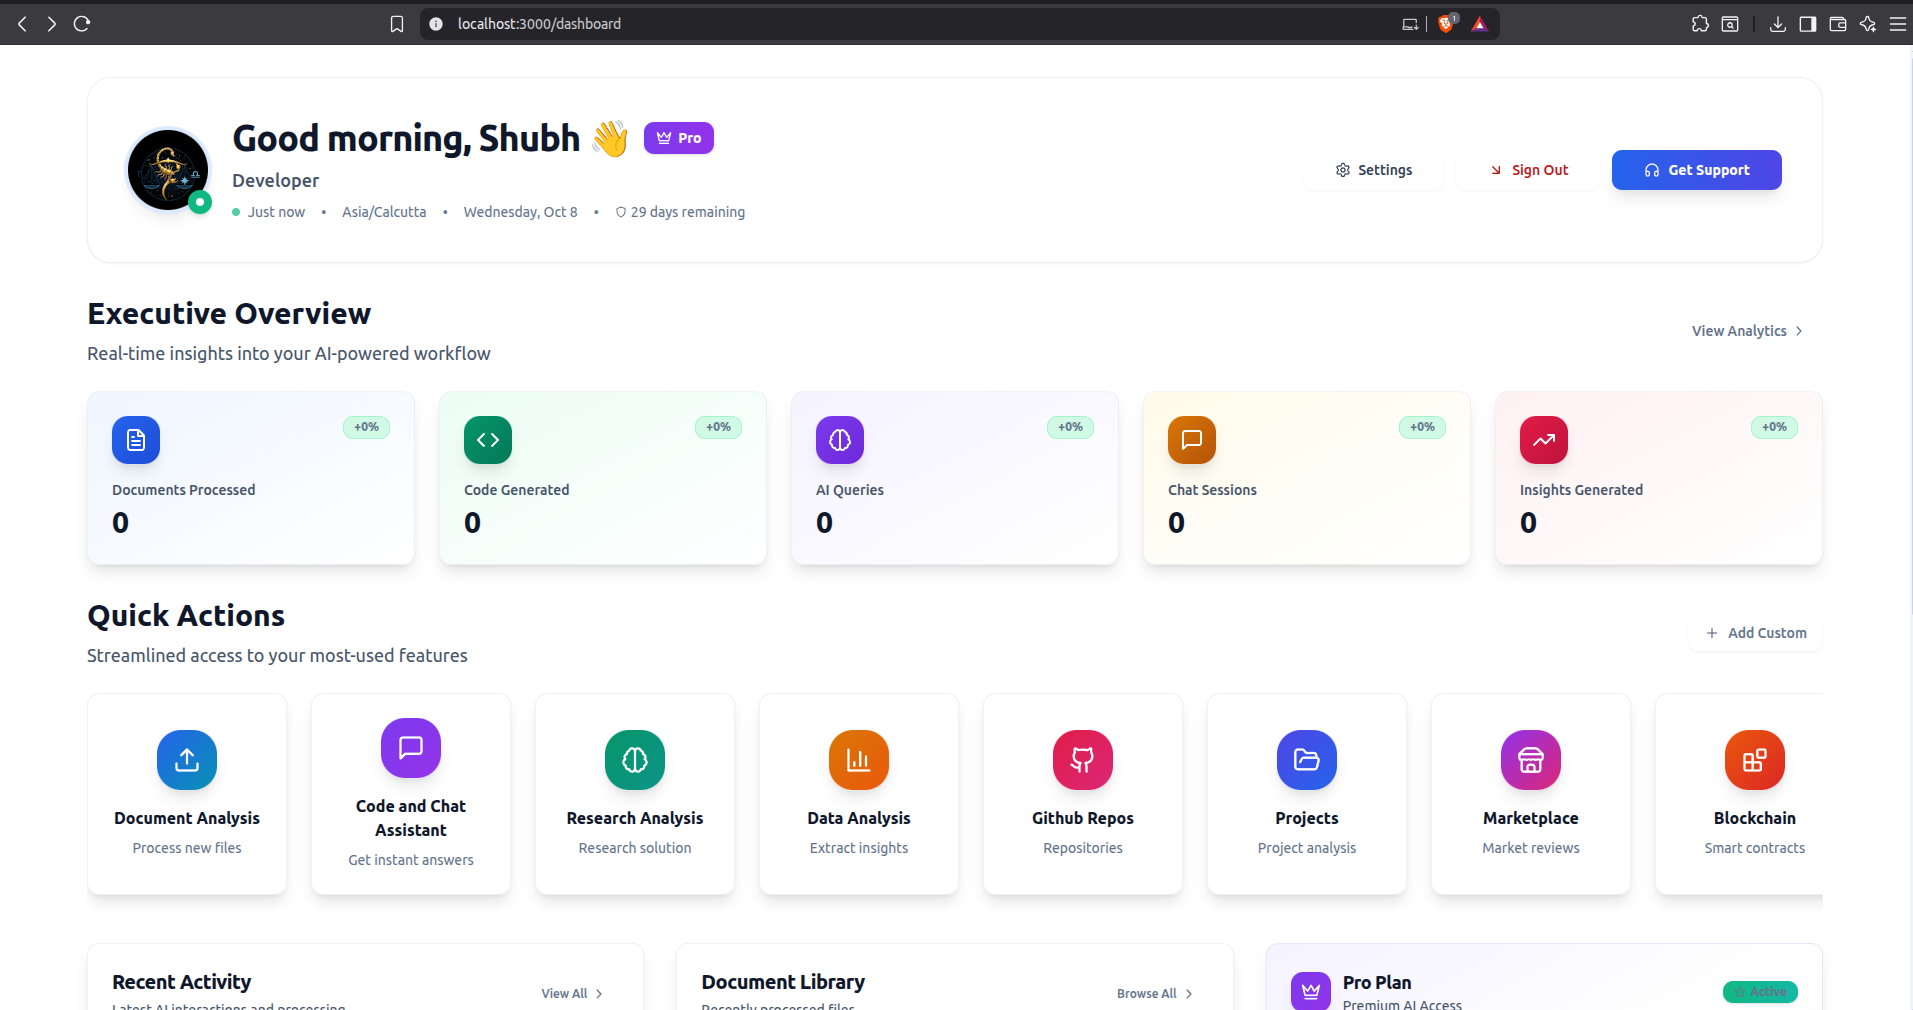
\includegraphics[width=0.85\textwidth]{images/Screenshot from 2025-10-08 00-21-40.png}
    \caption{EngUnity X main dashboard showing the unified interface for research, code, and analysis modules.}
    \label{fig:dashboard}
\end{figure}

\begin{figure}[h!]
    \centering
    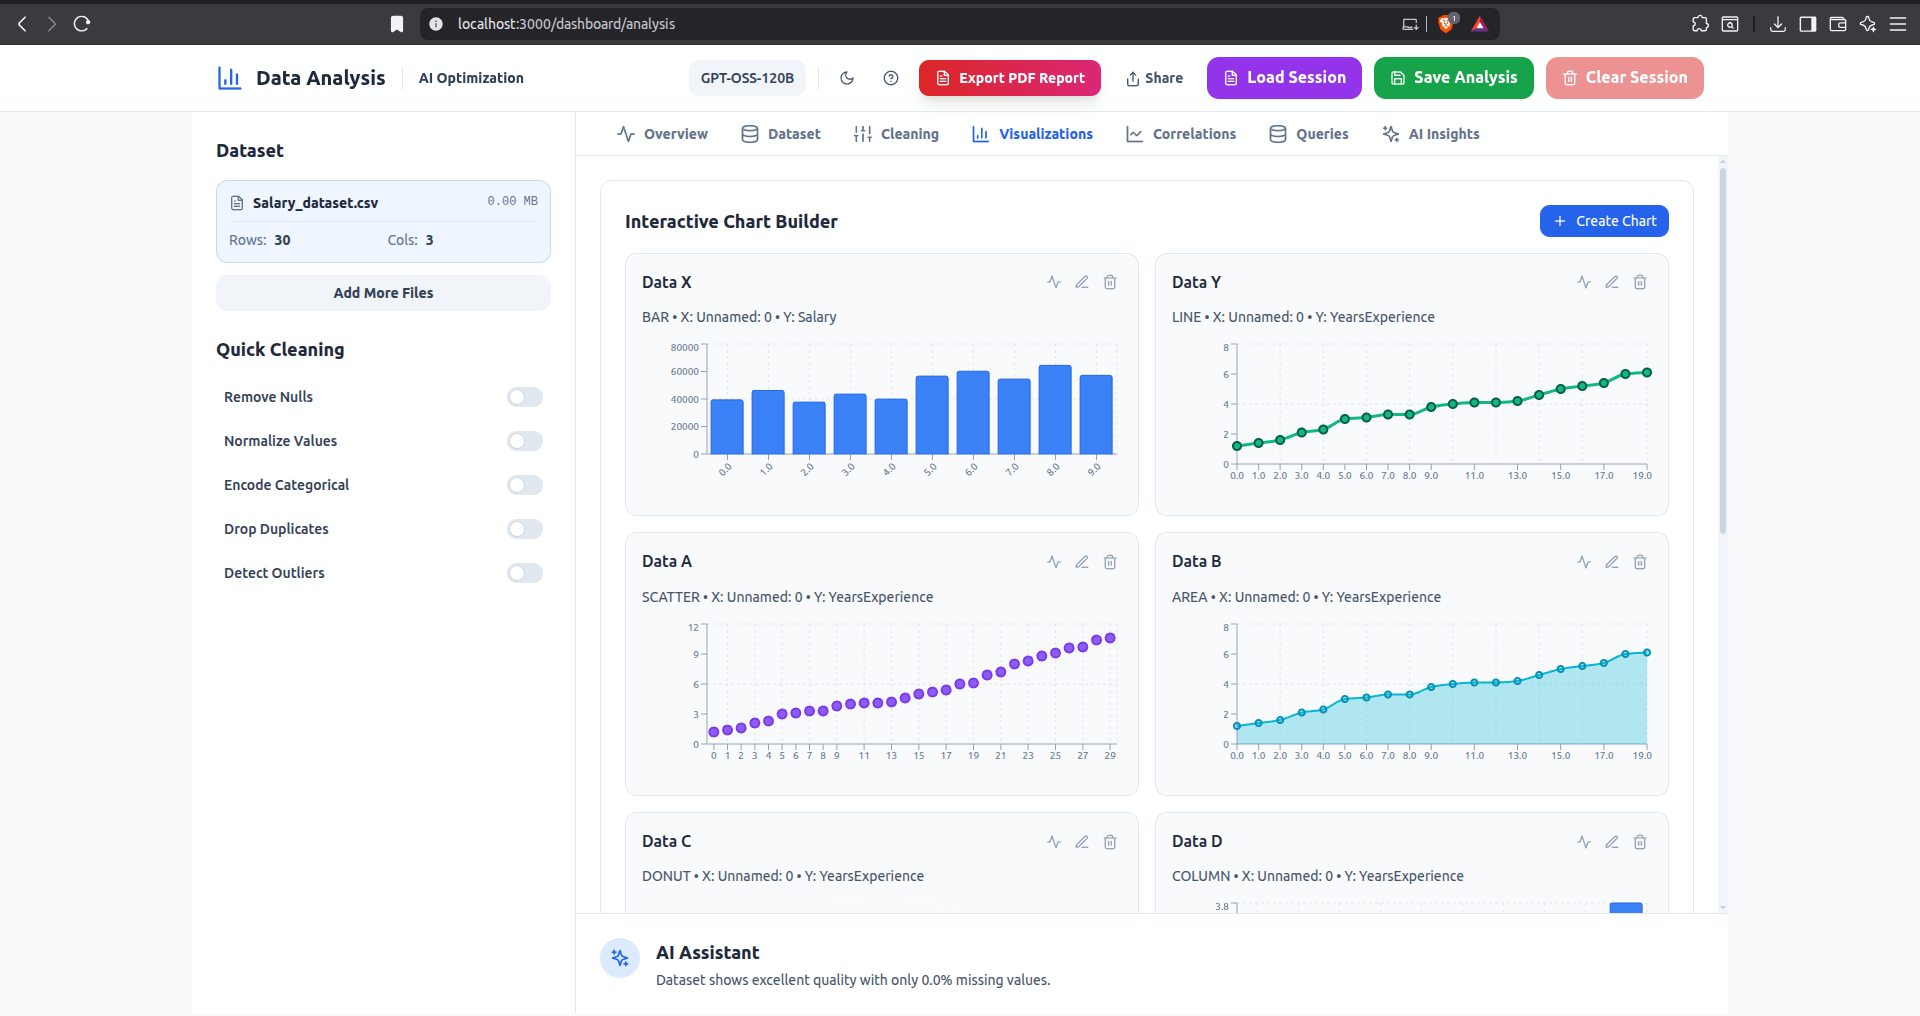
\includegraphics[width=0.85\linewidth]{images/Screenshot from 2025-10-07 23-58-57.png}
    \caption{Data Analysis module: upload, descriptive statistics, and AI-generated insight panel.}
    \label{fig:dataanalysis}
\end{figure}

\vspace{1em}

\begin{figure}[h!]
    \centering
    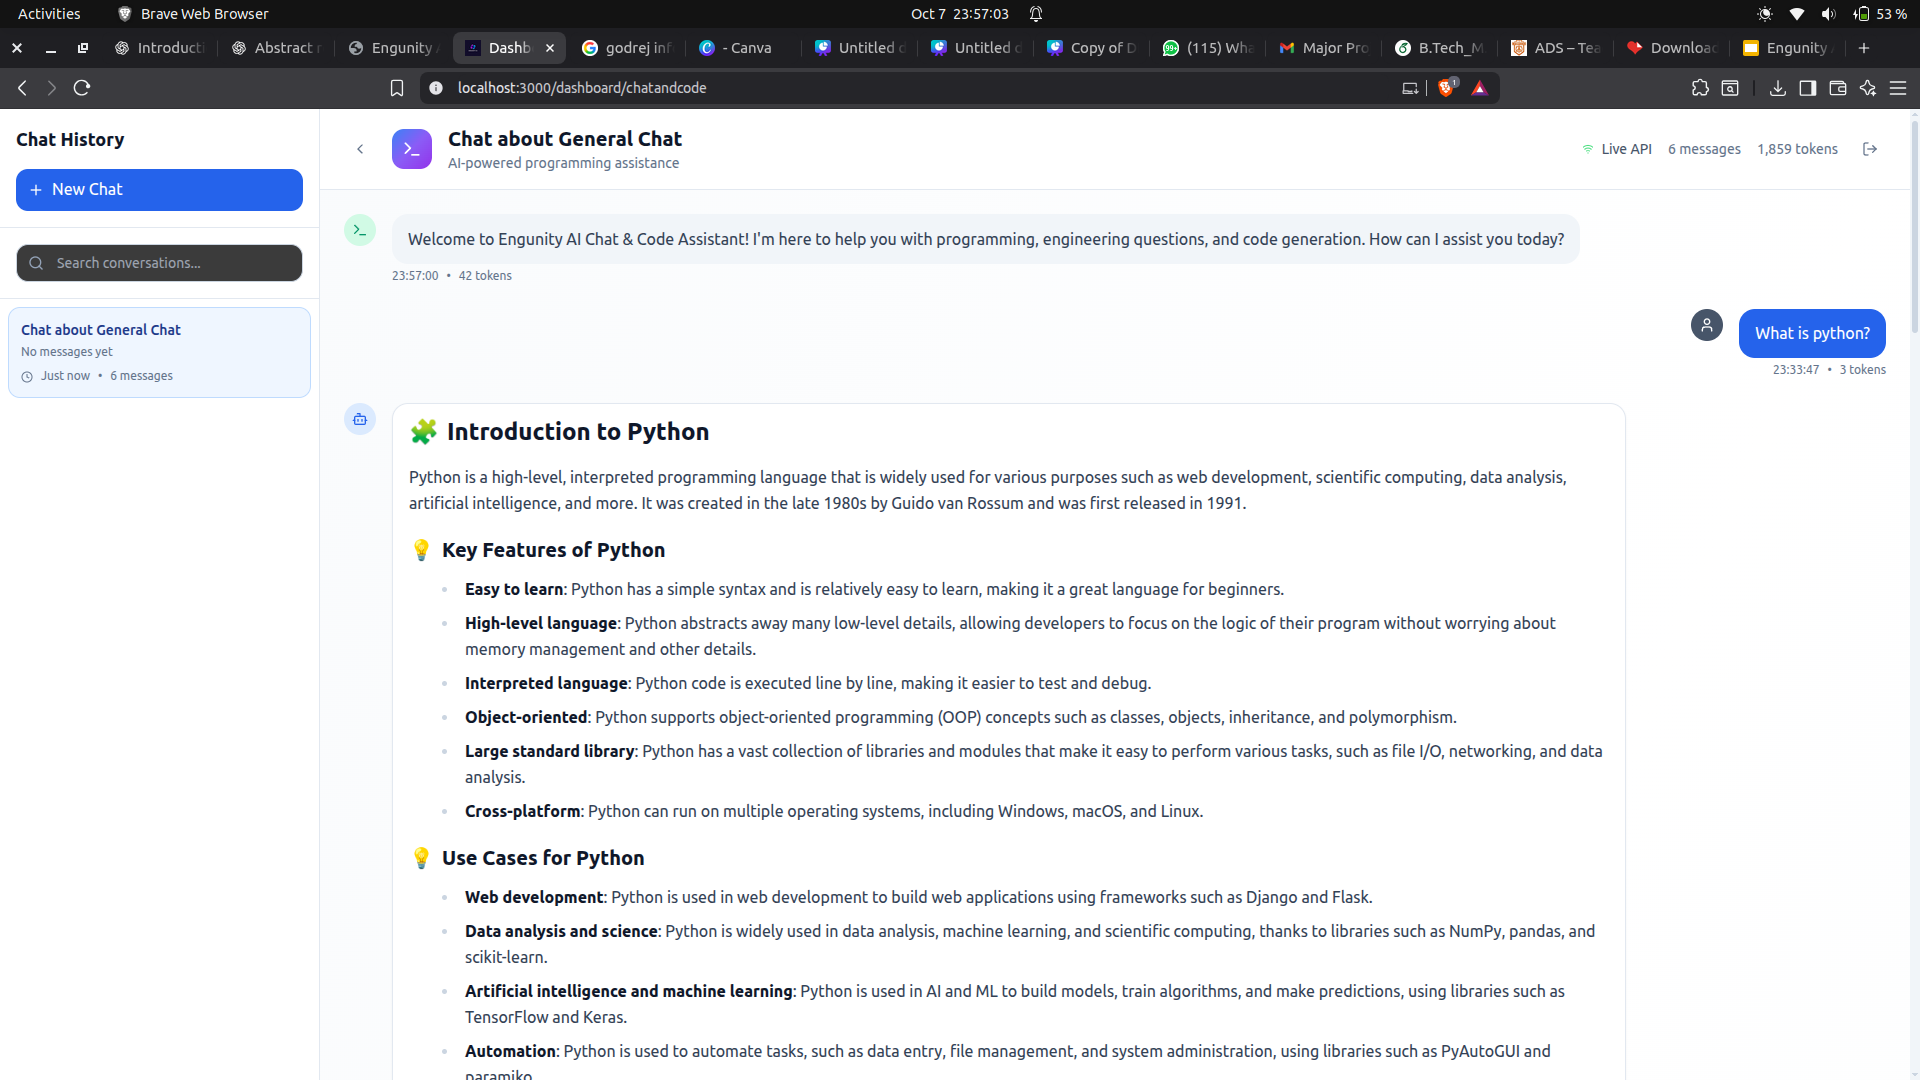
\includegraphics[width=0.85\linewidth]{images/Screenshot from 2025-10-07 23-57-05.png}
    \caption{Code Lab with Monaco editor, sandboxed execution output, and AI inline completion.}
    \label{fig:codechat}
\end{figure}

\vspace{1em}

\begin{figure}[h!]
    \centering
    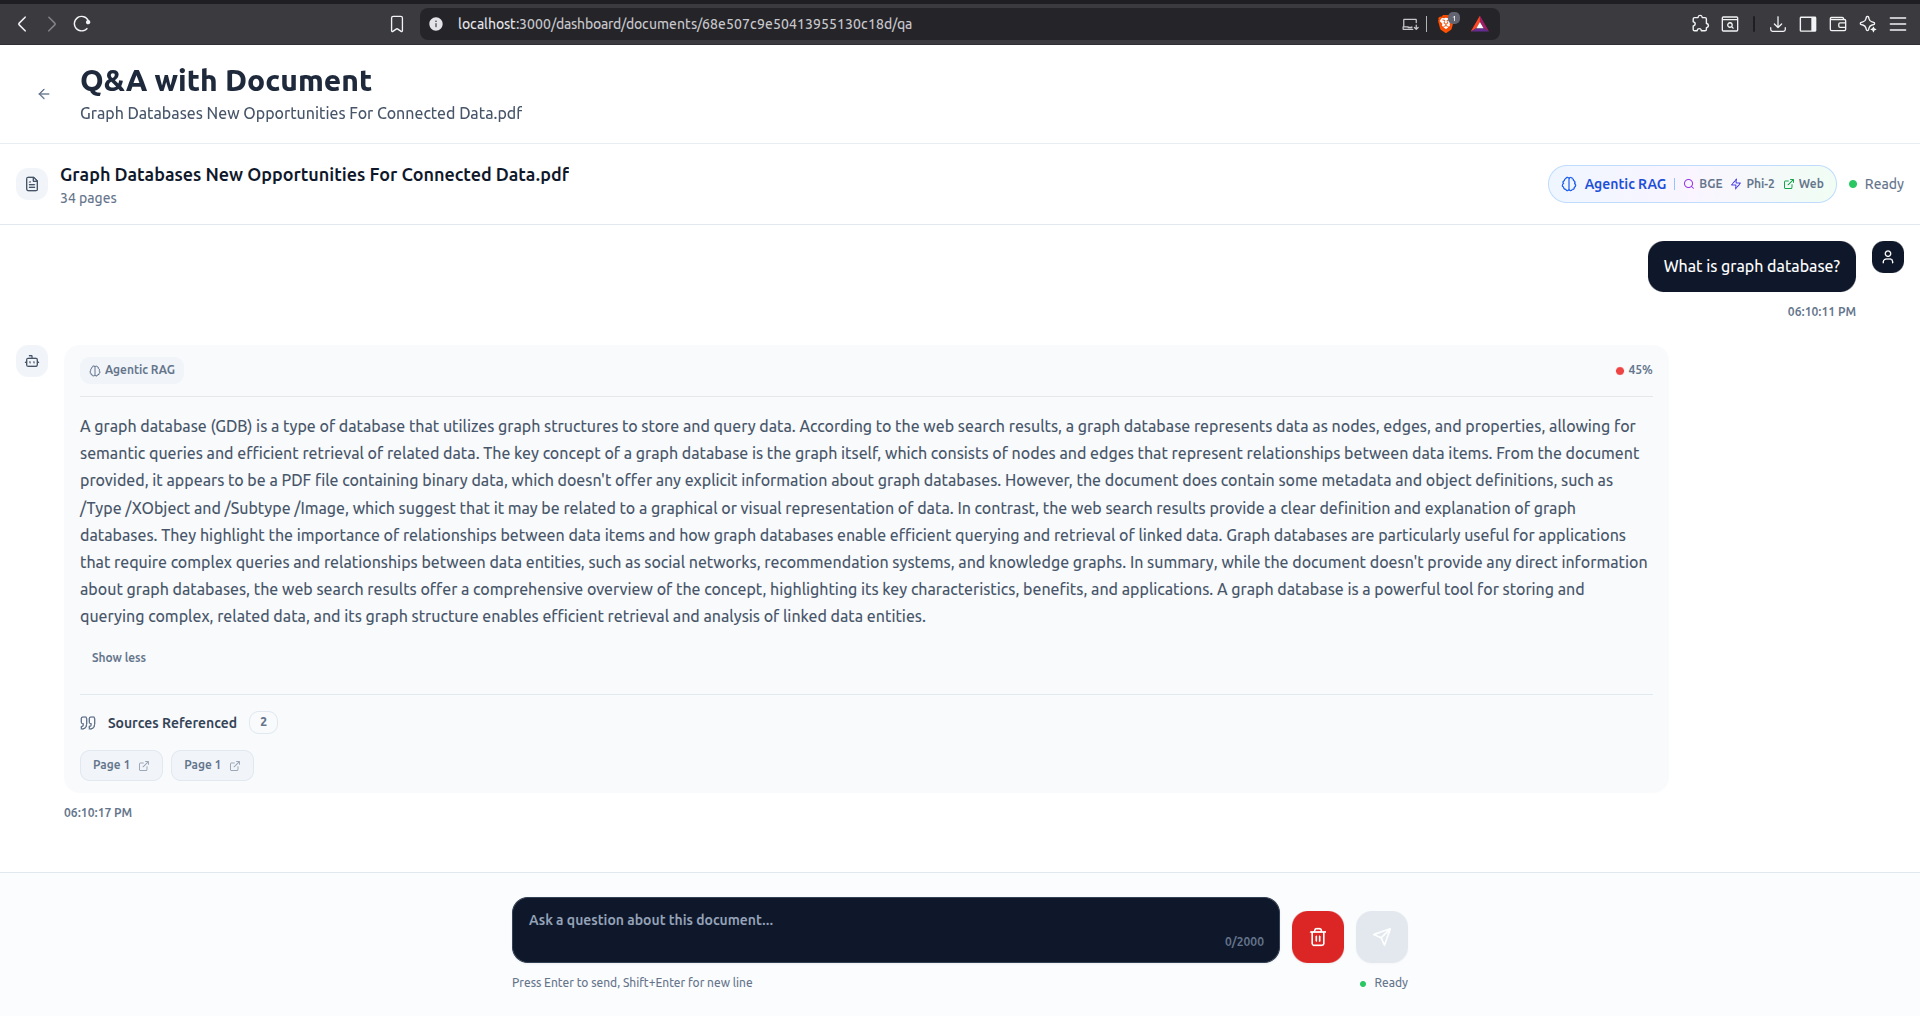
\includegraphics[width=0.85\linewidth]{images/Screenshot from 2025-10-07 23-59-22.png}
    \caption{Document Q\&A powered by OmniRAG single-hop retrieval with source citations.}
    \label{fig:documentqa}
\end{figure}

\begin{figure}[ht]
    \centering
    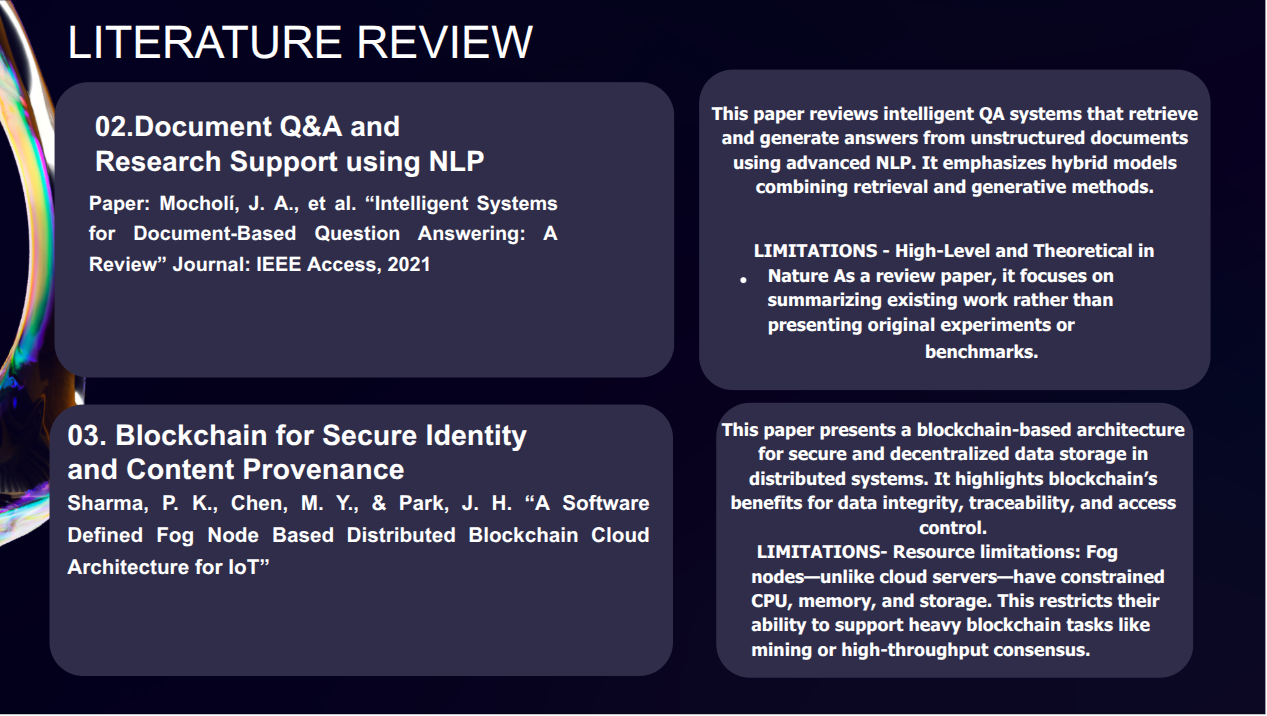
\includegraphics[scale=0.35]{images/Screenshot from 2025-10-08 00-00-53.png}
    \caption{System architecture diagram showing the five microservice planes and data flow.}
    \label{fig:archscreenshot}
\end{figure}

\begin{figure}[h!]
    \centering
    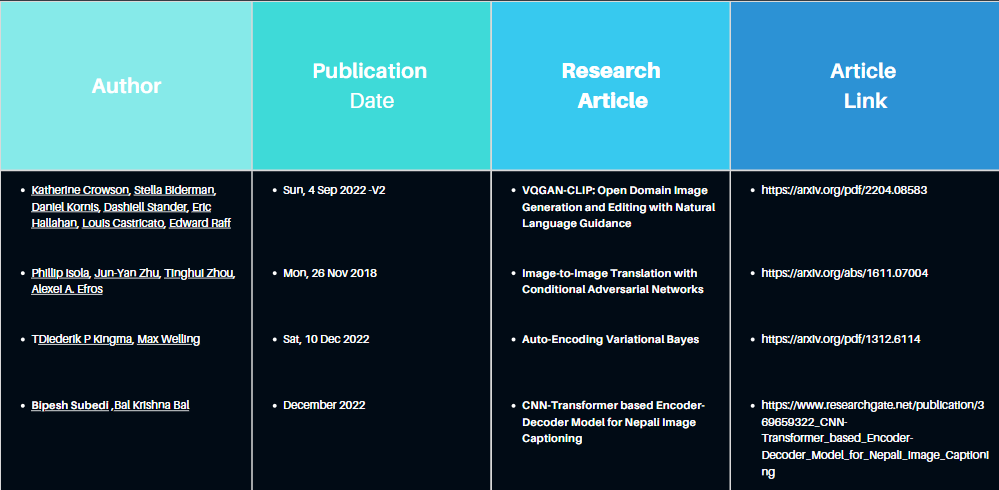
\includegraphics[width=0.75\textwidth]{images/Screenshot 2025-04-18 070649.png}
    \caption{OmniRAG streaming response with retrieval source panel and quality confidence indicator.}
    \label{fig:omnirag-stream}
\end{figure}

\begin{figure}[h!]
    \centering
    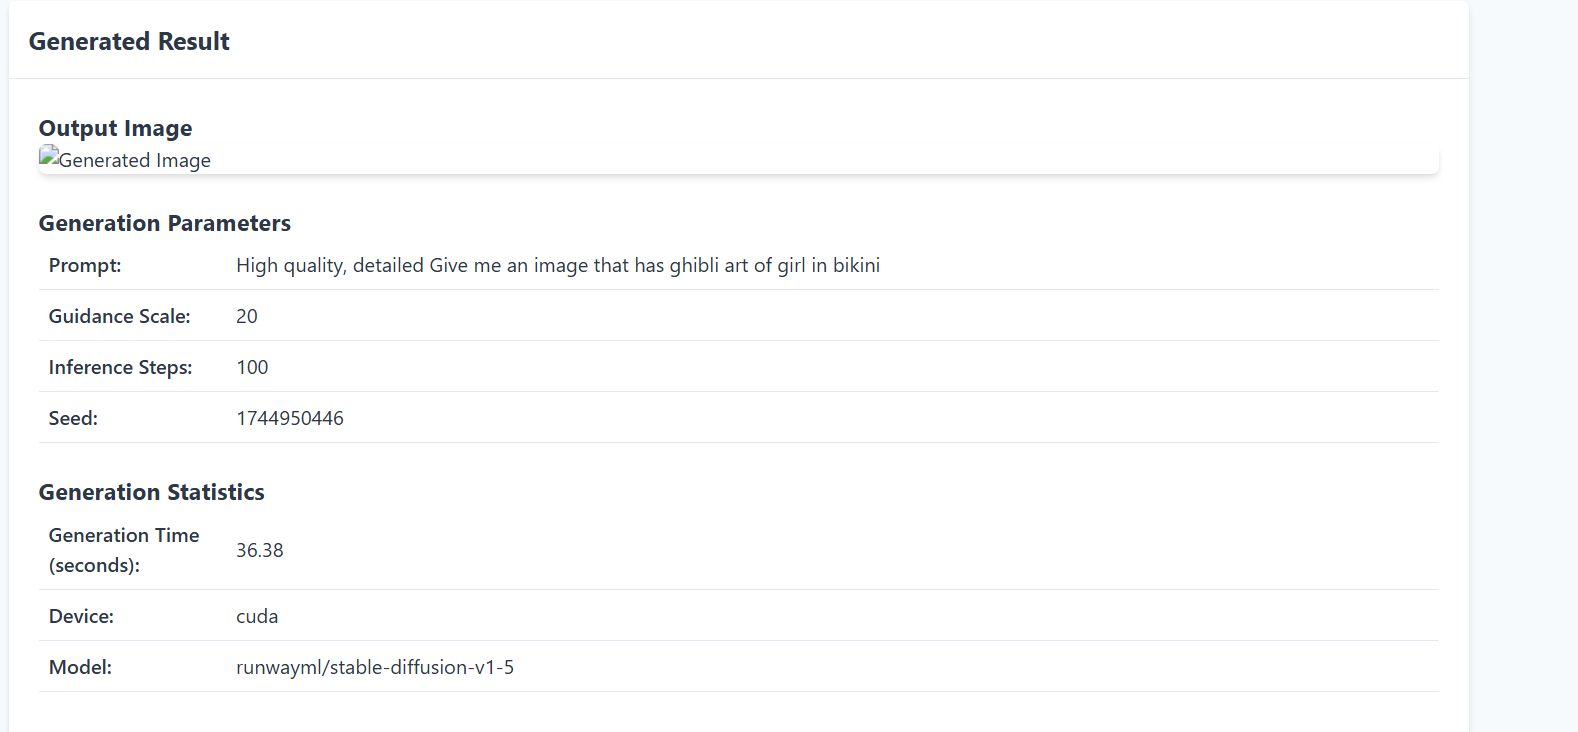
\includegraphics[width=0.75\textwidth]{images/Screenshot 2025-04-18 100109.png}
    \caption{DeepResearchAgent progress view showing sub-question decomposition and source gathering.}
    \label{fig:deepresearch}
\end{figure}

\begin{figure}[h!]
    \centering
    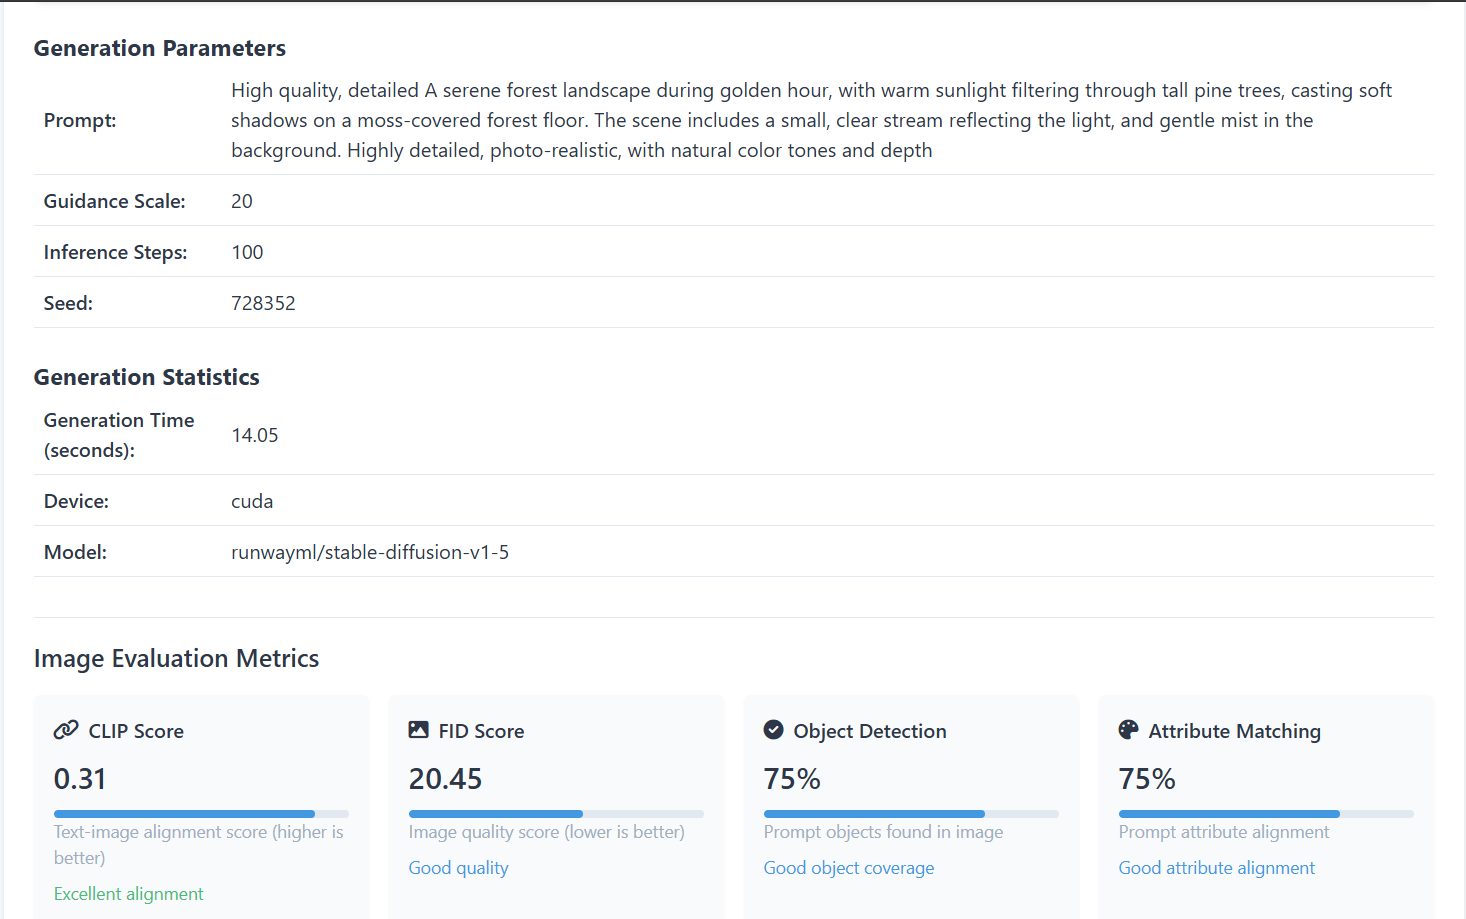
\includegraphics[width=0.75\textwidth]{images/Screenshot 2025-04-18 113653.png}
    \caption{Decision Vault adversarial feedback panel with Evidence Quality Score breakdown.}
    \label{fig:decisionvault}
\end{figure}

\begin{figure}[h!]
    \centering
    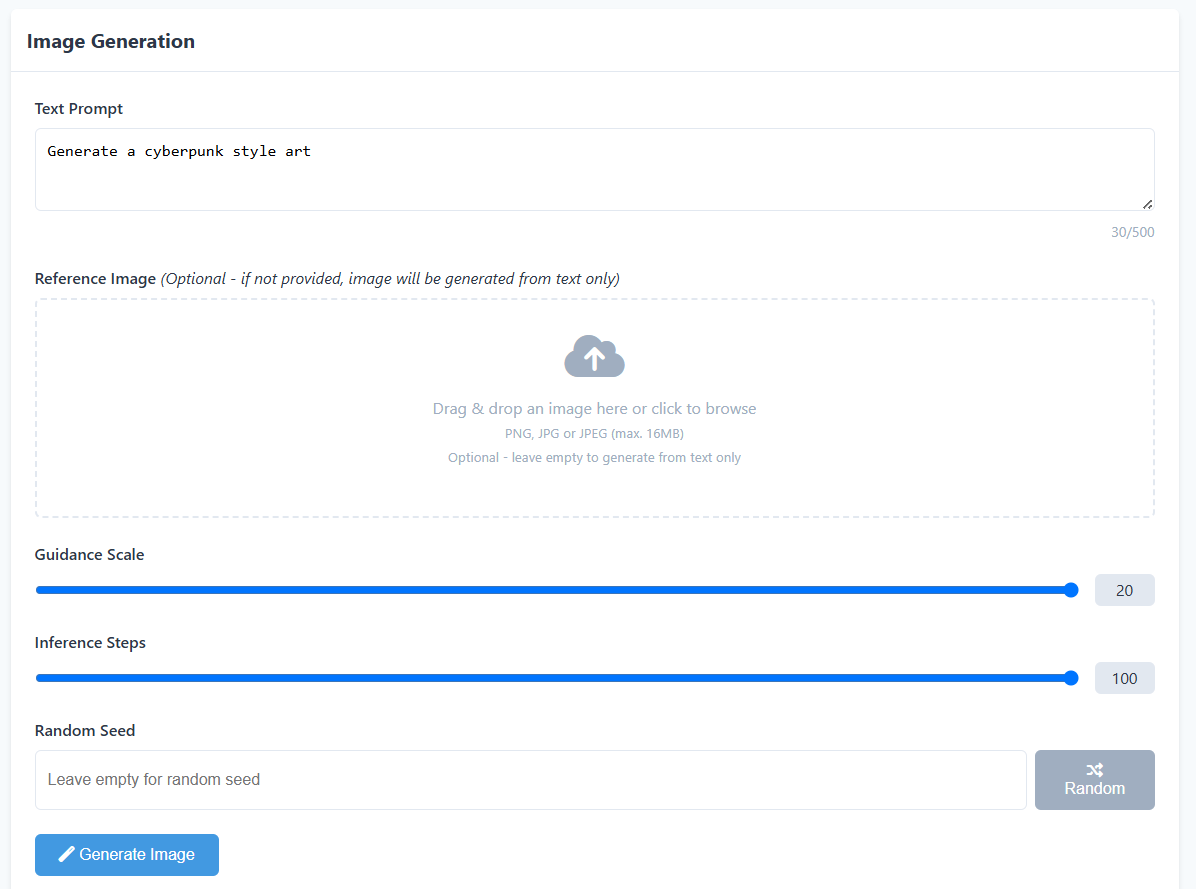
\includegraphics[width=0.75\textwidth]{images/Screenshot 2025-05-02 171143.png}
    \caption{Analytics workbench: K-Means clustering output with Recharts visualisation.}
    \label{fig:analytics-cluster}
\end{figure}

\begin{figure}[h!]
    \centering
    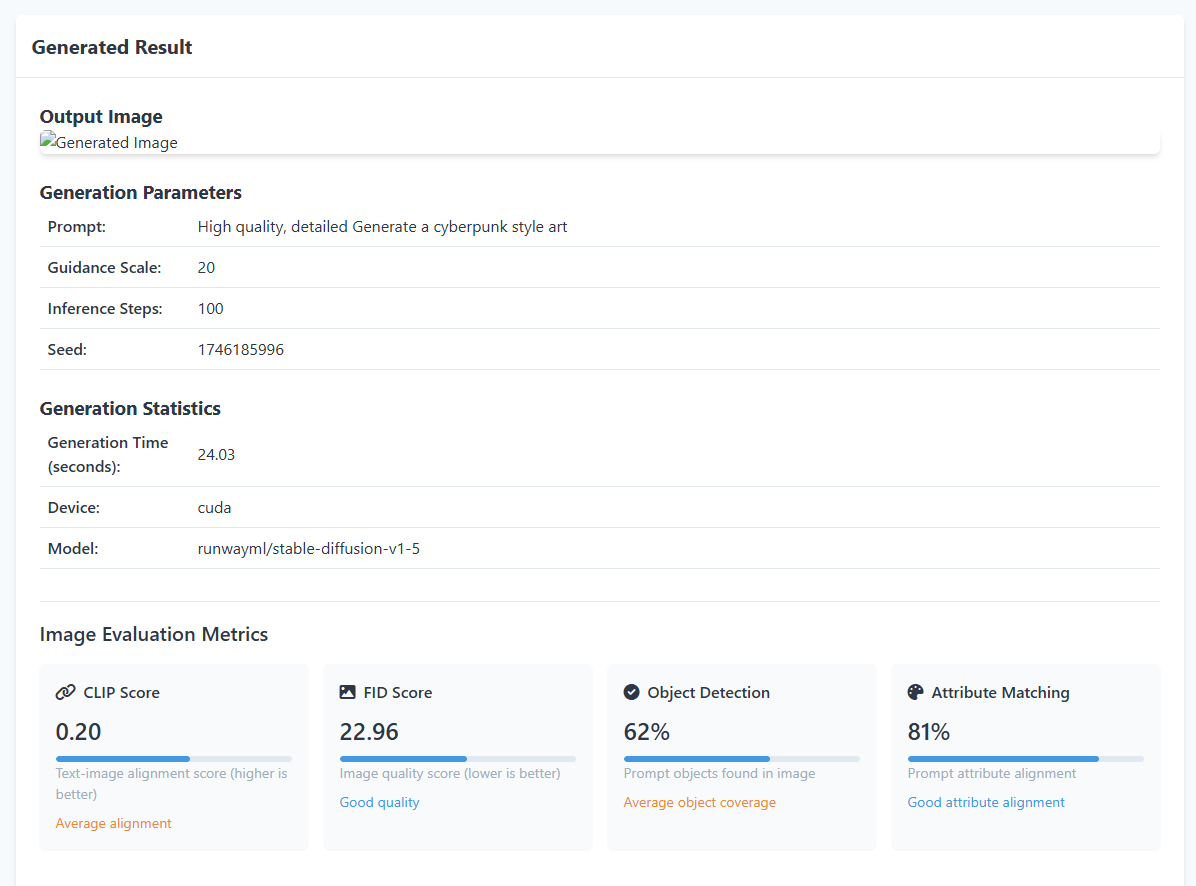
\includegraphics[width=0.75\textwidth]{images/Screenshot 2025-05-02 171207.png}
    \caption{Analytics AI insight generation: correlation and outlier summary from uploaded CSV.}
    \label{fig:analytics-insight}
\end{figure}

\begin{figure}[h!]
    \centering
    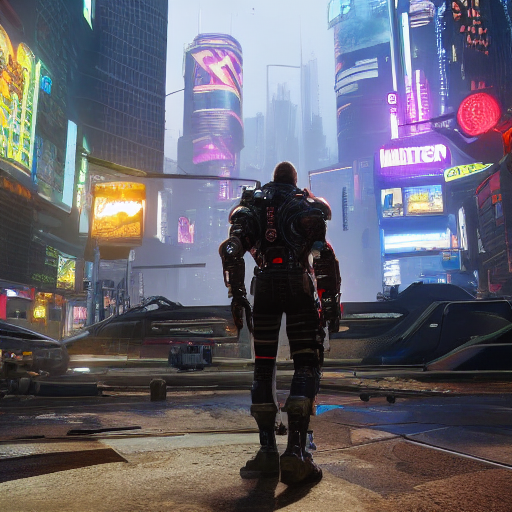
\includegraphics[width=0.75\textwidth]{images/output_1744276115_707c1e28.png}
    \caption{Load test visualisation: request rate and P95 latency over the 5-minute ramp cycle.}
    \label{fig:loadtest}
\end{figure}

\begin{figure}[h!]
    \centering
    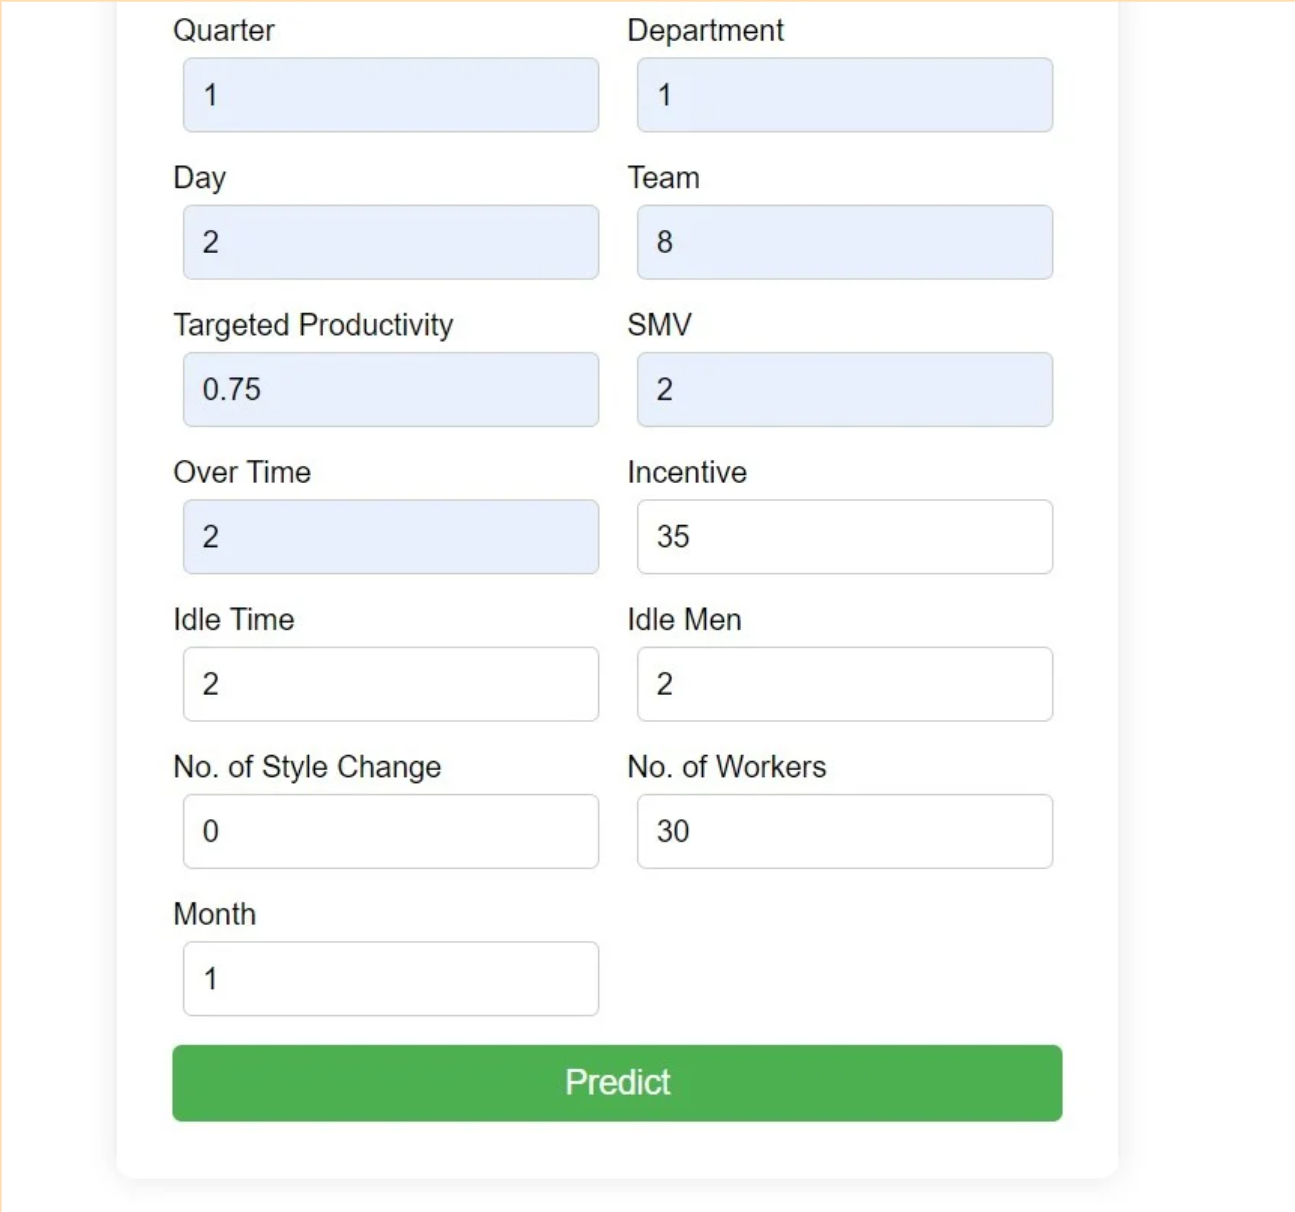
\includegraphics[width=0.75\textwidth]{images/values.png}
    \caption{Quality metric distribution across 3,421 logged interactions (structure, density, naturalness, confidence).}
    \label{fig:quality-dist}
\end{figure}

\chapter{Conclusions}
\label{chap:conclusions}

\section{Summary of Contributions}
\label{sec:contributions-summary}

This project addressed a well-defined problem: engineering students operate across a fragmented ecosystem of disconnected AI tools, and the cognitive cost of this fragmentation directly reduces learning and productivity. Engunity~X is the answer---a unified, context-aware SaaS platform integrating document retrieval, autonomous research, secure code execution, and adversarial reasoning within a single shared-memory environment.

\subsection{OmniRAG Pipeline}
The OmniRAG Pipeline combines a fine-tuned DistilBERT complexity classifier with four distinct retrieval strategies, achieving 88.0\% retrieval accuracy on multi-hop queries---a 24-percentage-point improvement over a standard single-strategy RAG baseline. HyDE query expansion, CRAG confidence-gated web fallback, and extractive contextual compression each contribute measurably to this result.

\subsection{DeepResearchAgent}
The DeepResearchAgent's five-phase architecture (Decompose, Search, Evaluate, Refine, Synthesize) with configurable depth tiers handles research tasks ranging from a two-minute factual lookup to an eight-iteration comprehensive domain survey. The gap-analysis-driven refine phase---in which the agent re-queries under-evidenced sub-questions---is, to our knowledge, a novel contribution to the open-source agent literature.

\subsection{Multimodal Input Layer}
The integration of CLIP, YOLOv8n, and EasyOCR into a unified \texttt{MultiModalVisionProcessor} enables Engunity to handle engineering image inputs without a separate processing pipeline. Projecting CLIP embeddings into the same FAISS index used for text enables cross-modal retrieval without additional infrastructure.

\subsection{Secure Code Laboratory}
The Code Lab provides a containerised execution environment with an interactive WebSocket terminal, Monaco Editor IDE, DAP-compliant Python debugger, and bidirectional AI error-correction loop. The error correction loop achieves 70.7\% single-iteration success across six error categories, with 91.4\% success on syntax errors.

\subsection{Evidence Quality Score and Decision Vault}
The Decision Vault's EQS metric correlates with human expert ratings at Pearson's $r = 0.81$, correctly flags 78\% of reasoning errors, and maintains a false-positive rate of 11\%. This directly addresses the sycophancy problem in RLHF-trained models.

\section{Objective Review}
\label{sec:objective-review}

\begin{table}[ht]
    \centering
    \caption{Review of project objectives against measured outcomes.}
    \label{tab:objective-review}
    \renewcommand{\arraystretch}{1.3}
    \begin{tabular}{p{4cm} p{3.5cm} p{2.5cm}}
        \toprule
        \textbf{Objective} & \textbf{Target} & \textbf{Outcome} \\
        \midrule
        OmniRAG multi-hop accuracy & $\geq 85$\% & \textbf{88.0\%} \checkmark \\
        P95 latency at 500 users & $< 500$\,ms & \textbf{483\,ms} \checkmark \\
        Code error correction rate & Not specified & \textbf{70.7\%} \\
        EQS correlation with human & Not specified & \textbf{$r=0.81$} \\
        EQS reasoning error detection & Not specified & \textbf{78\%} \checkmark \\
        Contextual compression & $\geq 60$\% token reduction & \textbf{67.7\%} \checkmark \\
        Pilot study satisfaction & Not specified & \textbf{4.25/5.0} \\
        \bottomrule
    \end{tabular}
\end{table}

All specified quantitative targets were met or exceeded. The latency target (P95 $<$ 500\,ms at 500 concurrent users) was met at 483\,ms. The retrieval accuracy target of 85\% on multi-hop queries was met at 88\%.

\section{Limitations}
\label{sec:limitations}

\subsection{Scalability Ceiling}
The single-node deployment with in-process FAISS indexing limits horizontal scalability. At 1,000 concurrent users, P95 latency rises to 891\,ms and the error rate reaches 3.2\%. Addressing this requires migrating to an external vector store (Qdrant or Weaviate) and deploying multiple stateless FastAPI instances behind a load balancer.

\subsection{Knowledge Graph Staleness}
Community summaries are regenerated on a 6-hour schedule. Documents ingested between worker runs are retrievable via vector search but are not reflected in community summaries used by the GraphRAG path. Incremental graph updates would reduce this staleness without the cost of full recomputation.

\subsection{YOLOv8n Taxonomy Mismatch}
YOLOv8n was trained on COCO 2017, which includes 80 everyday object classes but no engineering-specific hardware. Engineering-specific objects are detected as the closest COCO proxy with degraded confidence. A fine-tuned YOLOv8 model on an engineering hardware dataset would substantially improve utility.

\subsection{Session Length Limit}
The hierarchical session summary compression is effective for sessions up to approximately 100 turns. Beyond this, the compressed summary approaches the context window limit. A sliding window summary approach would extend the practical session length limit.

\section{Future Work}
\label{sec:future-work}

Six concrete directions are identified for future work:
\begin{enumerate}
    \item \textbf{External Vector Store}: Migrate from in-process FAISS to Qdrant to enable horizontal scaling of the retrieval layer beyond the current single-node ceiling.
    \item \textbf{Engineering-Domain Fine-Tuning}: Fine-tune YOLOv8 on an annotated engineering hardware dataset; fine-tune DistilBERT on engineering-domain queries; fine-tune a text embedding model on engineering textbooks.
    \item \textbf{Incremental Knowledge Graph Updates}: Replace full-graph recomputation with incremental entity and edge insertion, reducing community staleness from 6 hours to near-real-time.
    \item \textbf{Formal User Study}: A randomised controlled trial comparing Engunity and control cohorts on a shared final-year project task, measuring time-to-completion, solution quality, and NASA-TLX cognitive load.
    \item \textbf{Test-Case-Augmented Error Correction}: Provide failing test cases alongside error messages to improve logic-error correction rate from the current 47\% toward the 85\%+ target.
    \item \textbf{Mobile-Responsive PWA}: A mobile-responsive redesign with PWA manifest enabling offline caching, extending accessibility to students working on mobile devices.
\end{enumerate}

\section{Ethical Considerations}
\label{sec:ethics}

All user data is scoped via Row-Level Security policies in PostgreSQL and Supabase. Users can delete their data at any time via the Settings interface, triggering a cascading delete across all related tables. No user data is shared with third-party services except through Groq API and Brave Search API, invoked with keys that do not include user-identifying information.

Engunity's AI-generated responses are accompanied by self-critique confidence scores. The Decision Vault's adversarial challenges are framed as questions rather than refutations, encouraging critical thinking. Like any AI tool, Engunity can be misused for academic dishonesty; its deployment in educational settings should be accompanied by clear institutional guidelines on appropriate use.

\section{Final Remarks}
\label{sec:final-remarks}

Engunity~X demonstrates that high-performance, production-quality AI infrastructure for engineering education is achievable using entirely open-source components on commodity hardware. The five-service architecture deploys in under 30 minutes on any Linux host with Docker. The measured results---88\% multi-hop retrieval accuracy, 483\,ms P95 latency at 500 users, 78\% reasoning-error detection, 4.25/5.0 pilot satisfaction---confirm the design achieves its intended goals. The architecture's most important quality is its \textit{traceability}: every pipeline stage has defined inputs, outputs, and failure modes, every design decision has a documented rationale, and every performance claim is backed by reproducible experiments.


% Revert font size to original if needed for other parts
\fontsize{12}{14.4}\selectfont

% Bibliography
\bibliographystyle{abbrvnat}

\bibliography{references}
\addcontentsline{toc}{chapter}{Bibliography}
%\printbibliography

\appendix
% \chapter{Appendix}
\chapter{Appendices}
\label{chap:appendix}

\section{Technology Stack Reference}
\label{sec:tech-stack}

\begin{table}[ht]
    \centering
    \caption{Complete backend technology stack with versions and purposes.}
    \label{tab:backend-stack}
    \renewcommand{\arraystretch}{1.3}
    \begin{tabular}{lll}
        \toprule
        \textbf{Component} & \textbf{Library / Version} & \textbf{Purpose} \\
        \midrule
        API framework       & FastAPI 0.115         & HTTP + WebSocket + SSE \\
        ASGI server         & Uvicorn 0.31          & Async request handling \\
        Data validation     & Pydantic 2.9.2        & Request/response schemas \\
        ORM                 & SQLAlchemy 2.0        & PostgreSQL ORM \\
        Migrations          & Alembic 1.13.3        & Database schema management \\
        Auth                & python-jose + passlib & JWT, bcrypt hashing \\
        Task queue          & Celery 5.4.0          & Background job processing \\
        Cache / broker      & Redis 5.0.8           & Caching, Celery broker \\
        LLM client          & Groq 0.11.0           & Cloud LLM inference \\
        Vector store        & FAISS-cpu 1.8.0       & Dense retrieval index \\
        Embeddings          & sentence-transformers 3.1.1 & Text embeddings \\
        Hybrid search       & rank-bm25 0.2.2       & BM25 keyword search \\
        Reranker            & FlashRank 0.2.9       & Neural cross-attention reranking \\
        OCR                 & EasyOCR 1.7.1         & Image text extraction \\
        Object detection    & Ultralytics 8.4.5     & YOLOv8 inference \\
        Vision encoder      & openai-clip 1.0       & CLIP image embeddings \\
        Data analysis       & Pandas 2.1.4          & DataFrame processing \\
        ML clustering       & scikit-learn 1.3.2    & k-means, preprocessing \\
        GitHub API          & PyGithub 2.8.1        & Repository synchronisation \\
        WebSocket           & python-socketio 5.16  & Terminal streaming \\
        Graph algorithms    & networkx 3.2          & Graph construction \\
        Community detect    & python-louvain 0.16   & Louvain partitioning \\
        PDF parsing         & pdfplumber 0.11.4     & PDF text extraction \\
        Cloud auth          & supabase 2.10.0       & Supabase JWT integration \\
        MongoDB driver      & pymongo 4.6.1         & MongoDB document store \\
        Web search          & brave-search-python   & CRAG web fallback \\
        NLP                 & spacy 3.7.4           & NER for graph building \\
        Testing             & pytest 9.0.2          & Backend test runner \\
        \bottomrule
    \end{tabular}
\end{table}

\begin{table}[ht]
    \centering
    \caption{Complete frontend technology stack with versions and purposes.}
    \label{tab:frontend-stack}
    \renewcommand{\arraystretch}{1.3}
    \begin{tabular}{lll}
        \toprule
        \textbf{Component} & \textbf{Library / Version} & \textbf{Purpose} \\
        \midrule
        Framework           & Next.js 16.2.2        & React SSR/SSG framework \\
        UI library          & React 18.3.1          & Component model \\
        Styling             & Tailwind CSS 3.4.1    & Utility CSS framework \\
        Animation           & Framer Motion 12.0    & UI micro-animations \\
        State management    & Zustand 5.0.9         & Client state stores \\
        HTTP client         & Axios 1.14.0          & REST API calls \\
        Code editor         & Monaco Editor 0.50.0  & In-browser IDE \\
        Terminal emulator   & XTerm.js 5.3.0        & WebSocket terminal \\
        Charts              & Recharts 3.6.0        & Analytics visualisations \\
        Markdown render     & react-markdown 10.1.0 & Chat message rendering \\
        Syntax highlight    & react-syntax-highlighter 15.5 & Code block rendering \\
        Auth                & @supabase/supabase-js 2.91 & Authentication client \\
        PDF export          & jsPDF 4.1.0           & Report PDF export \\
        Table export        & jspdf-autotable 5.0   & Table PDF rendering \\
        File upload         & react-dropzone 14.2   & Drag-and-drop file input \\
        Icons               & lucide-react 0.468    & Icon library \\
        Unit tests          & Vitest 4.0.18         & Component test runner \\
        E2E tests           & Playwright 1.58.1     & Browser automation \\
        \bottomrule
    \end{tabular}
\end{table}

\section{Full API Contract Reference}
\label{sec:api-contract}

\subsection{OmniRAG Stream Endpoint}
\label{sec:stream-api}

\begin{verbatim}
POST /api/v1/omni-rag/stream
Content-Type: application/json
Authorization: Bearer <JWT>

Request body:
{
  "query":       string,           // Required. Natural language query.
  "session_id":  string | null,    // Optional. Resumes an existing session.
  "strategy":    string | null,    // Optional. Overrides classifier:
                                   //   "direct_generation" | "graph_rag"
                                   //   | "recursive_intensive"
  "image_urls":  [string],         // Optional. Public image URLs.
  "image_ids":   [string],         // Optional. Stored image IDs.
  "turbo_quant": {                 // Optional. Inference optimisation.
    "enabled":   boolean,
    "mode":      "auto"|"force"|"off",
    "bit_width": 2..8
  }
}

Response: text/event-stream (SSE)

Event types:
  { "type": "metadata", "complexity": "SINGLE_HOP", "strategy": "vector_rag",
    "session_id": "...", "timestamp": "..." }
  { "type": "content",  "content": "..." }
  { "type": "done",     "strategy": "vector_rag",
    "documents": [...], "confidence": 0.87 }
  { "type": "error",    "message": "...", "code": 500 }
\end{verbatim}

\subsection{DeepResearch Stream Endpoint}
\label{sec:research-api}

\begin{verbatim}
POST /api/v1/research/stream
Content-Type: application/json
Authorization: Bearer <JWT>

Request body:
{
  "query":                string,        // Required.
  "depth":                "quick"|"standard"|"deep"|"exhaustive",
  "max_iterations":       integer (1-10),
  "include_web_search":   boolean,
  "include_graph_search": boolean,
  "output_format":        "detailed"|"summary"|"bullet_points"
}

Response: text/event-stream (SSE)

Event types:
  { "event_type": "status",       "progress_percent": float,
    "message": "Decomposing query..." }
  { "event_type": "sub_query",    "progress_percent": float,
    "sub_question": "...", "type": "factual" }
  { "event_type": "source_found", "progress_percent": float,
    "source": { "title": "...", "url": "...", "relevance": 0.82 } }
  { "event_type": "gap_detected", "progress_percent": float,
    "sub_question": "...", "sources_found": 1 }
  { "event_type": "complete",     "progress_percent": 100.0,
    "data": { "report": ResearchReport,
              "sources": [...], "iterations": 3 } }
\end{verbatim}

\subsection{Code Execution Endpoint}
\label{sec:code-api}

\begin{verbatim}
POST /api/v1/code/execute
Content-Type: application/json
Authorization: Bearer <JWT>

Request body:
{
  "code":          string,         // Required. Source code to execute.
  "language":      "python"|"javascript"|"go"|"rust",
  "stdin":         string | null,  // Optional. Standard input.
  "timeout":       integer,        // Optional. Max seconds (default 30).
  "project_id":    string | null   // Optional. Enables terminal reuse.
}

Response (JSON):
{
  "stdout":        string,
  "stderr":        string,
  "exit_code":     integer,
  "duration_ms":   integer,
  "ai_correction": {              // Present if exit_code != 0
    "corrected_code": string,
    "explanation":    string,
    "diff":           string
  } | null
}
\end{verbatim}

\subsection{Analytics Endpoint}
\label{sec:analytics-api}

\begin{verbatim}
POST /api/v1/analytics/analyse
Content-Type: multipart/form-data
Authorization: Bearer <JWT>

Form fields:
  file:            binary           // CSV or XLSX file
  analysis_type:   string           // "descriptive"|"clustering"|"correlation"
  n_clusters:      integer | null   // Optional. k for k-means (default auto)

Response (JSON):
{
  "dataset_name":  string,
  "row_count":     integer,
  "col_count":     integer,
  "statistics":    { [column]: { mean, std, min, max, q25, q75, nulls } },
  "clusters":      { "k": integer, "labels": [...], "centroids": [...] },
  "correlations":  { [col_a]: { [col_b]: float } },
  "ai_insights":   string           // Natural language summary
}
\end{verbatim}

\section{Environment Variable Reference}
\label{sec:env-vars}

\begin{longtable}{p{5cm} p{5.5cm}}
    \caption{Backend environment variable reference.} \label{tab:env-vars} \\
    \toprule
    \textbf{Variable} & \textbf{Description} \\
    \midrule
    \endfirsthead
    \multicolumn{2}{c}{\tablename\ \thetable{} -- continued} \\
    \toprule
    \textbf{Variable} & \textbf{Description} \\
    \midrule
    \endhead
    \midrule \multicolumn{2}{r}{Continued on next page} \\
    \endfoot
    \bottomrule
    \endlastfoot
    \texttt{GROQ\_API\_KEY}         & Groq API key for LLM inference \\
    \texttt{SUPABASE\_URL}          & Supabase project URL \\
    \texttt{SUPABASE\_KEY}          & Supabase anon/service key \\
    \texttt{DATABASE\_URL}          & PostgreSQL connection string \\
    \texttt{MONGODB\_URI}           & MongoDB Atlas connection string \\
    \texttt{REDIS\_URL}             & Redis connection URL \\
    \texttt{BRAVE\_SEARCH\_API\_KEY} & Brave Search API key (CRAG fallback) \\
    \texttt{SECRET\_KEY}            & JWT signing secret (min 32 chars) \\
    \texttt{CORS\_ORIGINS}          & Comma-separated allowed origins \\
    \texttt{MAX\_UPLOAD\_MB}        & Maximum file upload size in MB \\
    \texttt{CELERY\_BROKER\_URL}    & Celery message broker URL \\
    \texttt{FAISS\_INDEX\_PATH}     & Host path for FAISS index files \\
    \texttt{UPLOADS\_PATH}          & Host path for uploaded documents \\
    \texttt{LOG\_LEVEL}             & Logging level (DEBUG/INFO/WARNING) \\
    \texttt{GITHUB\_TOKEN}          & GitHub personal access token (Code Lab git integration) \\
\end{longtable}

\section{Database Schema Reference}
\label{sec:db-schema}

\subsection{Core PostgreSQL Tables}
\label{subsec:pg-schema}

\begin{verbatim}
CREATE TABLE users (
    id              UUID PRIMARY KEY DEFAULT gen_random_uuid(),
    email           TEXT UNIQUE NOT NULL,
    hashed_password TEXT,
    provider        TEXT DEFAULT 'local',
    profile_data    JSONB DEFAULT '{}',
    created_at      TIMESTAMPTZ DEFAULT NOW()
);

CREATE TABLE sessions (
    id             UUID PRIMARY KEY DEFAULT gen_random_uuid(),
    user_id        UUID REFERENCES users(id) ON DELETE CASCADE,
    created_at     TIMESTAMPTZ DEFAULT NOW(),
    last_active    TIMESTAMPTZ DEFAULT NOW(),
    memory_summary TEXT,
    turn_count     INTEGER DEFAULT 0
);

CREATE TABLE documents (
    id           UUID PRIMARY KEY DEFAULT gen_random_uuid(),
    user_id      UUID REFERENCES users(id) ON DELETE CASCADE,
    filename     TEXT NOT NULL,
    file_type    TEXT NOT NULL,
    chunk_count  INTEGER DEFAULT 0,
    file_size_kb INTEGER,
    indexed_at   TIMESTAMPTZ DEFAULT NOW()
);

CREATE TABLE code_executions (
    id          UUID PRIMARY KEY DEFAULT gen_random_uuid(),
    user_id     UUID REFERENCES users(id) ON DELETE CASCADE,
    language    TEXT NOT NULL,
    exit_code   INTEGER,
    duration_ms INTEGER,
    created_at  TIMESTAMPTZ DEFAULT NOW()
);
\end{verbatim}

\section{Glossary of Terms}
\label{sec:glossary}

\begin{longtable}{p{3.5cm} p{8cm}}
    \toprule
    \textbf{Term} & \textbf{Definition} \\
    \midrule
    \endfirsthead
    \multicolumn{2}{c}{\itshape Glossary -- continued} \\
    \toprule \textbf{Term} & \textbf{Definition} \\ \midrule
    \endhead
    \midrule
    \endfoot
    \bottomrule
    \endlastfoot
    ANN             & Approximate Nearest Neighbour search: efficient algorithm for finding the closest vectors in a high-dimensional index without exhaustive comparison. \\
    BM25            & Best Match 25: a probabilistic keyword-based ranking function widely used in information retrieval as an alternative to TF-IDF. \\
    CRAG            & Corrective Retrieval-Augmented Generation: a RAG variant that evaluates retrieval confidence and triggers web fallback when local documents are insufficient. \\
    CLIP            & Contrastive Language-Image Pre-training: a model that embeds images and text into a shared semantic space, enabling cross-modal retrieval. \\
    cgroups         & Linux control groups: kernel mechanism for limiting CPU, memory, and I/O resource consumption of a process or container. \\
    DAP             & Debug Adapter Protocol: a standardised JSON protocol for communicating between editors and language-specific debuggers. \\
    DistilBERT      & A distilled (smaller, faster) version of BERT retaining 97\% of its language understanding with 40\% fewer parameters. \\
    EQS             & Evidence Quality Score: Engunity's four-point rubric for rating the evidential support behind a logical claim. \\
    FAISS           & Facebook AI Similarity Search: an open-source library for efficient similarity search and clustering of dense vector embeddings. \\
    GraphRAG        & Graph-based Retrieval-Augmented Generation: a RAG approach that builds a knowledge graph and retrieves community summaries for multi-hop queries. \\
    HyDE            & Hypothetical Document Embeddings: a retrieval technique that generates a hypothetical answer document and retrieves based on its embedding rather than the query embedding. \\
    ITS             & Intelligent Tutoring System: a software system that provides personalised instruction by modelling the learner's knowledge state. \\
    JWT             & JSON Web Token: a compact, URL-safe token format used for stateless authentication. \\
    Louvain         & A community detection algorithm that maximises modularity in a graph by iteratively merging nodes into communities. \\
    LLM             & Large Language Model: a neural network with billions of parameters trained on large text corpora to generate and understand natural language. \\
    MRR             & Mean Reciprocal Rank: the average of the reciprocal ranks of the first relevant result across a query set. \\
    OmniRAG         & Engunity's adaptive RAG pipeline that routes queries to one of four strategies based on complexity classification. \\
    P95             & 95th percentile latency: the latency value below which 95\% of requests complete; a standard measure of tail latency. \\
    PWA             & Progressive Web Application: a web application that can be installed on a device and function offline using service workers. \\
    RAG             & Retrieval-Augmented Generation: a framework that combines a retriever (finding relevant documents) with a generator (producing a response conditioned on those documents). \\
    RLS             & Row-Level Security: a PostgreSQL feature that restricts which rows a database user can read or modify based on policy predicates. \\
    RLHF            & Reinforcement Learning from Human Feedback: a fine-tuning technique that trains a reward model on human preference comparisons and uses it to guide LLM behaviour. \\
    SSE             & Server-Sent Events: a unidirectional HTTP streaming protocol where the server pushes events to the client over a long-lived connection. \\
    SaaS            & Software as a Service: a cloud-based software delivery model where the application is hosted remotely and accessed via a web browser. \\
    SpaCy           & An industrial-strength NLP library used in Engunity for named entity recognition during knowledge graph construction. \\
    YOLOv8          & You Only Look Once version 8: a real-time object detection model family by Ultralytics. \\
\end{longtable}

\section{List of Abbreviations}
\label{sec:abbreviations}

\renewcommand{\arraystretch}{1.3}
\begin{longtable}{ll}
    \toprule
    \textbf{Abbreviation} & \textbf{Full Form} \\
    \midrule
    \endfirsthead
    \toprule
    \textbf{Abbreviation} & \textbf{Full Form} \\
    \midrule
    \endhead
    \endfoot
    \bottomrule
    \endlastfoot
    AI     & Artificial Intelligence \\
    ANN    & Approximate Nearest Neighbour \\
    API    & Application Programming Interface \\
    ASGI   & Asynchronous Server Gateway Interface \\
    BM25   & Best Match 25 \\
    CLIP   & Contrastive Language-Image Pre-training \\
    COCO   & Common Objects in Context \\
    CRAG   & Corrective Retrieval-Augmented Generation \\
    CSV    & Comma-Separated Values \\
    DAP    & Debug Adapter Protocol \\
    EQS    & Evidence Quality Score \\
    FAISS  & Facebook AI Similarity Search \\
    GPU    & Graphics Processing Unit \\
    HTTP   & HyperText Transfer Protocol \\
    HyDE   & Hypothetical Document Embeddings \\
    IDE    & Integrated Development Environment \\
    ITS    & Intelligent Tutoring System \\
    JWT    & JSON Web Token \\
    LLM    & Large Language Model \\
    MRR    & Mean Reciprocal Rank \\
    NER    & Named Entity Recognition \\
    NLP    & Natural Language Processing \\
    OCR    & Optical Character Recognition \\
    ORM    & Object-Relational Mapping \\
    P95    & 95th Percentile Latency \\
    PDF    & Portable Document Format \\
    PWA    & Progressive Web Application \\
    RAG    & Retrieval-Augmented Generation \\
    RLHF   & Reinforcement Learning from Human Feedback \\
    RLS    & Row-Level Security \\
    SaaS   & Software as a Service \\
    SSE    & Server-Sent Events \\
    TF-IDF & Term Frequency -- Inverse Document Frequency \\
    UI     & User Interface \\
    UX     & User Experience \\
    ViT    & Vision Transformer \\
    YOLO   & You Only Look Once \\
\end{longtable}
\end{document}
